\documentclass[uplatex,openany,oneside,a4j,11pt]{jsbook}
\usepackage[top=25truemm,bottom=25truemm,left=25truemm,right=25truemm]{geometry}
\usepackage[dvipdfmx]{graphicx}
\graphicspath{{./img/}}
\usepackage[dvipdfmx]{color}
\usepackage[dvipdfmx,colorlinks,linkcolor=blue,urlcolor=blue,bookmarks=true,bookmarksnumbered=true]{hyperref}
\usepackage{pxjahyper}
\usepackage{bookmark}
\usepackage{url}
\usepackage{booktabs}
\usepackage{amsmath}
\usepackage{amssymb}
\usepackage{amsfonts}
\usepackage{here}
\usepackage{comment}
\usepackage{subfigure}
\usepackage{braket}
\usepackage{caption}

\def\inner<#1,#2>{\langle #1|#2 \rangle}
%\def\outer<#1>{\rangle #1 \langle}

%\usepackage{mediabb}
%\addbibresource{'C:/Users/miyao/Desktop/MasterThesis/bibs'}
%\usepackage{physics}
\usepackage[style=phys,articletitle=true,biblabel=brackets,chaptertitle=false,pageranges=false,backend=biber]{biblatex}
\addbibresource{bibs.bib}
\begin{document}
\begin{titlepage}
    \begin{center}
        {\Large 2020 年度 修士論文}\\
        \vspace{180truept}
        {\Huge 超伝導量子ビット間における\\
        \vspace{10truept}
        CZゲートの研究}\\
        \vspace{70truept}

        {\Large \today}\\

        \vspace{70truept}

        {\Large 東京理科大学大学院 理学研究科物理学専攻 蔡研究室\\
        (学籍番号 1219506)}\\

        \vspace{20truept}

        {\huge 亥埜 創太}\\

        \vspace{160truept}
        {\Large 東京理科大学大学院 理学研究科物理学専攻}\\
    \end{center}
\end{titlepage}
\addcontentsline{toc}{chapter}{序章}

\section*{序章}

現在のコンピュータを上回る計算性能を秘めているとして近年注目を集めている量子コンピュータは、大規模化・高精度化が進んでいる。非常に限定された分野においてのみではあるが、ここ数年ではスーパーコンピュータが100年以上掛かって解ける問題を数分の間に解けるような実機も登場している。
一昨年、53個の超伝導量子ビットを実装した量子計算機によるQuantum supremacy(量子超越性)がGoogleの研究チームにより報告された。
\cite{arute2019quantum} またこちらは実装手段に光を用いているが、昨年12月に中国の研究グループによりガウシアンボソンサンプリングという問題に関しての量子超越性が報告された。\cite{zhong2020quantum}\\
量子コンピュータ内で行われる計算の方式には大きく分けて2通りが存在する。
その一つのゲート型方式は、一個または複数個の量子ビットに対し「量子ゲート」と呼ばれる演算を逐次実行し計算を行う。
もう一つはアニーリング方式とよばれる、解く問題をイジングモデルに帰着させそのエネルギーが最小となるパラメータを求める方式である。\\
前者のゲート型は、論理ゲートを用いる現在のNeumann型コンピュータに近い回路モデルで計算を行う。その演算の内容はすべて、1量子ビットに関する量子状態操作(ゲート)
及び2量子ビットゲートであるCZゲートに分解可能であることがわかっている。\\
原理の項で詳しく述べることになるが、超伝導量子ビットを用いたCZゲートは一定の条件の下、量子ビットの状態を電流パルスを用いて遷移させることで実現される。
その電流パルスの印加のしかたにより
本紙では、量子ビット数の拡張を行う上で鍵となる2量子ビット間CZゲートについて実装を試みるとともに、
行ったシミュレーション、及び超伝導体を用いて作成したサンプルに関する測定を行って得られた結果について報告する。
\setcounter{tocdepth}{2}
\tableofcontents
%\mainmatter
\chapter{目的}
    \begin{abstract}
    \end{abstract}
    \section{超伝導回路の大規模化}
    本研究の目的は共振器間の高強度結合素子の開発である。まずはこの研究のモチベーションについて説明することから始める。
    序章でも述べたが超伝導量子回路の集積度は年々向上しており、知名度の高い企業が研究開発に乗り出していることからも世間からの注目度は非常に高い。しかしながら、各々の量子ビットを効率よく相互作用させようとする際にはまだまだ課題も多い。超伝導量子回路を用いた大規模な集積回路として有名なのはD-wave社の量子アニーリング回路、Googleの万能型量子回路であるがその2つの例を見ても各々の量子ビットの全結合は実現できていない。量子ビットと結合素子を直接結合させるには回路デザインの観点から限界が生じている。我々の研究チームでは量子アニーリング型及び万能型のそれぞれについて2次元回路アーキテクチャの開発に取り組んでいる。この2つのアーキテクチャのうち特に量子アニーリング回路では本稿のテーマである。共振器間の高強度結合素子の開発が要となる。以下に大規模アニーリング回路を駆動するために必要なここの超伝導素子のパラメータを示す。

    この図には量子ビット間の実質的な結合強度Jijと量子ビットのパラメータが示されている。量子アニーリングはイジンぐモデルを前提に構築されたモデルであり、最終的な解は結合強度Jijにマッピングされる。始状態のパラメータは量子ビットの遷移周波数にマップされるため始状態と終状態において、この2つのパラメータはバランスがとれていることが前提となる。またスイープ時間において突発的な状態遷移を避けるために量子ビットの遷移周波数はGHz帯に設定する必要がある。この状況においてJijの強度をGHz体に保つためには共振器間の結合強度の絶対値には少なくとも400MHzが必要とされる。マッピングの自由度を上げるにはこのJijは正負でのバランスがとれていることが望ましい。
    以上より共振器間の結合に要請される理想的なパラメータは-400MHzから400MHzを自由に変調できるものである。
    先行研究\cite*{Wulschner2016}では-320MHzから37MHzの結合強度を実現しているが、正負両方向において強度不足であることがわかる。

\section{}

\section{結合振動子}
    本研究のテーマはエンジニアリングな側面が強いが、研究対象としている結合共振回路は物理モデルとしても非常に興味深い内容である。量子力学と古典力学のアナロジーとして連成振動子モデルは多くの研究がなされている。\cite*{Rodriguez2016}\cite*{Ivakhnenko2018}\cite*{Novotny2010}
    上記のモデルは一般的な共振素子(振動子)と共振素子を結合した系を理論的視点から論じている。今回作成した共振回路は共振器間のダイレクトな結合強度を変調できるという点で非常に魅力的である。一般的な共振素子はその遷移周波数がすべて同一であり、共振回路の周波数を持った光子を外部から入力しても高準位へと遷移してしまい、光子の放出現象は示さない。しかし、振動子間に結合項が存在すると振る舞いは一変し新たな固有モードが出現する。古典力学ではしばしばこのモードのことを基準モードと呼んでいる。この
    \begin{figure}[H]
        \centering
        \includegraphics[width=9cm]{b.pdf}
        \caption{エネルギースペクトル}
    \end{figure}
    \begin{figure}[H]
        \centering
        \includegraphics[width=9cm]{a.png}
        \caption{エネルギースペクトル}
    \end{figure}
    \begin{figure}[H]
        \centering
        \includegraphics[width=9cm]{c.pdf}
        \caption{エネルギースペクトル}
    \end{figure}




\chapter{原理}
    \begin{abstract}
    \end{abstract}
        本章ではまず、量子計算に用いられる一部の量子力学の公理について紹介する。
\section{量子ビット}
    \subsection{量子ビットの表現}
        古典コンピュータが電気信号のON,OFFを古典ビットの0,1に対応させるように、
        量子計算の基本単位を担う量子ビット(Quantum bit,略してQubitとも呼ばれる)は、ある量子系の固有状態をヒルベルト空間(内積を定義できるベクトル空間)$\mathcal{H}\in\mathbb{C}^2$上の
        \begin{equation}
            \ket{0}=\left(
                \begin{array}{c}
                  1\\
                  0\\
                \end{array}
              \right)
            ,
            \ket{1}=\left(
                \begin{array}{c}
                  0\\
                  1\\
                \end{array}
              \right)
        \end{equation}
        に対応させることで表現される。$\ket{0},\ket{1}$の元となる量子状態はスピンのアップ・ダウン、偏光の回転方向など様々にとることができるが
        本論文では後述する非線形調和振動子の光子数0個,1個の状態を$\ket{0}$,$\ket{1}$に対応させる。
        量子ビットの大きな特徴は、$\ket{0}$,$\ket{1}$の重ね合わせ状態が存在することである。
        状態$\ket{0}$,$\ket{1}$の確率振幅をそれぞれ$\alpha,\beta \leq 1$とすると1量子ビットの状態は
        \begin{equation}
            \ket{\psi}=\alpha\ket{0}+\beta\ket{1}
        \end{equation}
        と記述できる。1量子ビットの観測を行ったときに状態が$\ket{0}$に収束する確率は$|\alpha|^2$,$\ket{1}$に収束する確率は$|\beta|^2$であり
        $|\alpha|^2+|\beta|^2=1$を満たす。
        ()のように状態が基底ベクトル(この場合は{$\ket{0},\ket{1}$})の重ね合わせによって単位ベクトルで表現できるとき、この状態を純粋状態であるという。
        
        \subsubsection{ブロッホ球}
        先ほどの確率振幅による量子ビットの表現を視覚的に分かり易いものに置き換えてみる。
        適当な実数の位相$\gamma,\phi,\theta$を用いて、(2.2)は次のように書き換えられる。
        \begin{equation}
            \ket{\psi} =\mathrm{e}^{i\gamma}(\cos \frac{\theta}{2} \ket{0} +\mathrm{e}^{i\phi} \sin \frac{\theta}{2} \ket{1})
        \end{equation}
        全体にかかる位相である$\gamma$はゼロとして差し支えない。図のような
        \begin{figure}
            \begin{center}
                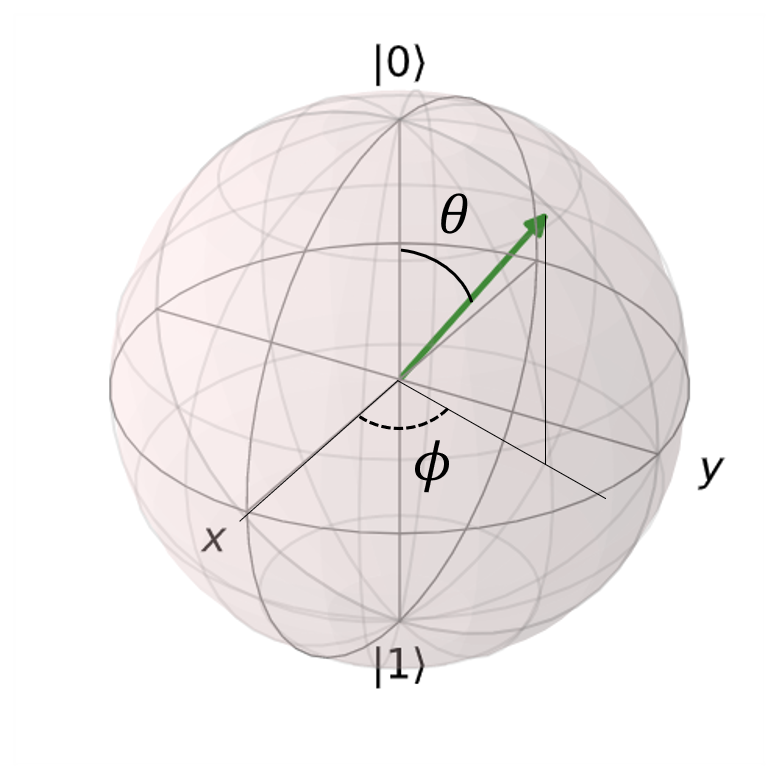
\includegraphics[width=5cm]{bloch.png}
                \caption{ブロッホ球}
            \end{center}
        \end{figure}
        $\ket{0}$を北極,$\ket{1}$を南極とした球を考えると、(2.3)は球面上のベクトルとして図示できる。
        このとき、$\theta$は状態ベクトルがz軸となす角、$\phi$はxy平面上に射影した状態ベクトルがx軸となす角とみなせる。
        状態ベクトルがx軸正方向に向くとき、$\ket{\psi} = \frac{(\ket{0}+\ket{1})}{\sqrt2}$であり、状態$\ket{0}$と$\ket{1}$が等確率で重ねあわされており($\ket{+}$状態)、y軸正方向を向くときには先ほどの重ね合わせ状態からz軸周りの位相が$\frac{\pi}{2}$変化した状態となる。($\ket{-}$状態)
        $\ket{0}$状態と$\ket{1}$状態の重ね合わせで表される純粋状態はすべてBloch球上の単位ベクトルとして表すことができる。

        \subsubsection{状態・期待値の測定}
        量子ビットの典型的な測定は{$\ket{0},\ket{1}$}による基底測定\footnote{測定に際して選ぶ基底は完全性を有する正規直交基底であれば何でもよいので,例として$\ket{+}$状態と$\ket{-}$状態の組み合わせを選ぶこともできる。}であり、測定により得られる状態は必ず0か1にランダムに収束する。
        状態が$\ket{\psi}$のとき、測定値i=0,1を得る確率は
        \begin{equation}
            P=|\inner<\psi,i>|^2
        \end{equation}
        で与えられる。このとき、先のブロッホ球における$\phi$、すなわち状態の位相の情報は失われる。このためブロッホ球上の$\phi$のみが異なる状態は測定によりすべて同じ状態として扱われる。\\
        また我々は量子ビットの状態だけでなく、準備した量子状態によって特定の物理量の期待値を測定するときがある。
        量子系における物理量はエルミート演算子$A$によって与えられ、状態$\ket{\psi}$のもとでの$A$の期待値$\langle A \rangle$は量子力学の公式より
        \begin{equation}
            \langle A \rangle =\langle \psi\ket{A\psi}
        \end{equation}
        で与えられる。

        \subsubsection{密度演算子}
        環境系との結合や複数の量子ビットが存在する状況下での1量子ビット状態には、混合状態という状態が存在する。
        例えば量子ビット$\ket{0}$,$\ket{1}$をそれぞれ1つずつ用意して箱に入れ、1つを取り出す場合、$\ket{0}$を取り出す確率、$\ket{1}$を取り出す確率はそれぞれ50\%である。
        しかしこの場合、取り出す1量子ビットの状態を重ね合わせを用いて$\ket{\psi} = \frac{(\ket{0}+\ket{1})}{\sqrt2}=\ket{+}$と書くことはできない。
        系全体で見たときに0,1の割合が50:50であることは既知であるが、1量子ビットについては0,1である確率がどのような割合で重ねあわされているか分からないためである。
        実際、状態$\ket{+}$は基底$\ket{+}$による測定で確率1を与えるが、上述の状態は必ず0か1かのどちらかであり、$\ket{+}$による測定でどちらの場合も確率1/2を与えるはずである。
        このような重ね合わせとは異なる、確率的に状態が与えられる状態を混合状態という。\\
        この混合状態を含めて量子ビットの状態を記述するために密度演算子というものを導入する。\\
        状態$\psi$のとりうる基底状態が$\{\ket{\psi_i}\}_{i=0}^N$であり、確率$p_i$で状態$\ket{\psi_i}$をとるとすると、その密度演算子$\rho$は
        \begin{equation}
            \rho_\psi=\sum_i^N p_i \ket{\psi_i}\bra{\psi_i}
        \end{equation}
        で与えられる。
        基底$\ket{\phi_0}$による状態$\rho_\psi$の測定結果は
        \begin{equation*}
            \bra{\phi_0}\rho_\psi\ket{\phi_0}
        \end{equation*}
        となる。また、物理量Aを状態$\rho$で測定した期待値は
        \begin{equation}
            \langle A \rangle =\mathrm{Tr}(\rho A)=\mathrm{Tr}(A\rho)
        \end{equation}
        で与えられる。\\
        先ほど例にあげた状態を密度演算子で記述すると、$p_0=1/2$, $p_1=1/2$より
        \begin{equation*}
            \rho=\frac{1}{2}\ket{0}\bra{0}+\frac{1}{2}\ket{1}\bra{1}
            =\left(
                \begin{array}{cc}
                  1/2 & 0\\
                  0 & 1/2\\
                \end{array}
              \right)
        \end{equation*}
        となり、$\bra{0}\rho\ket{0}=1/2$, $\bra{1}\rho\ket{1}=1/2$,さらに$\bra{+}\rho\ket{+}=1/2$であることから系の状態を正しく記述できている。
        重ね合わせ状態の密度演算子による表現は
        \begin{equation*}
            \rho=1\cdot\ket{+}\bra{+}
            =\left(
                \begin{array}{c}
                  1/\sqrt2\\
                  1/\sqrt2
                \end{array}
              \right)
              \left(
                \begin{array}{cc}
                  1/\sqrt2 & 1/\sqrt2  
                \end{array}
              \right)
            =\left(
                \begin{array}{cc}
                  1/2 & 1/2\\
                  1/2 & 1/2\\
                \end{array}
              \right)
        \end{equation*}
        となり、両者が明確に異なる状態であることがわかる。\\
        密度演算子は、いかなる状態の測定を行っても確率は0以上でありその総和は1という要請から
        \begin{eqnarray}
            \rho \geq 0 \\
            \mathrm{Tr}(\rho)=1
        \end{eqnarray}
        という性質を持つ。純粋状態に加え、単位ベクトルでは記述できない混合状態を表せる密度演算子は\\
        量子状態の最も一般的な表現を与える演算子である。

        \subsubsection{多量子ビット系の表現}
        ここでは2つ以上の量子ビットが存在する系(合成系)の表現について説明する。\\
        2つの量子ビットが存在しそれぞれの量子系にヒルベルト空間$\mathcal{H}_1,\mathcal{H}_2$が付随する場合、2量子ビット合成系に付随するヒルベルト空間$\mathcal{H}$は
        \begin{equation}
            \mathcal{H}=\mathcal{H}_1\otimes\mathcal{H}_2
        \end{equation}
        n量子ビット系なら
        \begin{equation}
            \mathcal{H}=\mathcal{H}_1\otimes\mathcal{H}_2\otimes\cdots\otimes\mathcal{H}_n
        \end{equation}
        に拡張される。ここで$\otimes$はテンソル積を表す。2量子ビット系の基底は互いの{$\ket{0},\ket{1}$}基底から1つずつを選んだ組み合わせのテンソル積を羅列し
        \begin{equation*}
            \ket{00}
            =\left(
                \begin{array}{c}
                    1 \\
                    0 \\
                    0 \\
                    0
                \end{array}
             \right),
            \ket{01}=\left(
                \begin{array}{c}
                    0 \\
                    1 \\
                    0 \\
                    0
                \end{array}
              \right),
            \ket{10}=\left(
                \begin{array}{c}
                    0 \\
                    0 \\
                    1 \\
                    0
                \end{array}
              \right),
            \ket{11}=\left(
                \begin{array}{c}
                    0 \\
                    0 \\
                    0 \\
                    1
                \end{array}
              \right)
        \end{equation*}
        となる。($\ket{\psi}\otimes\ket{\phi}$を$\ket{\psi\phi}$と略記する)\\
        状態については、互いの量子ビット間に後述する量子エンタングルメントがない場合、密度演算子$\rho_1,\rho_2$のテンソル積が合成系の状態
        \begin{equation}
        \begin{split}
            \rho &= \rho_1\otimes\rho_2\\
            \mathrm{両者が純粋状態} \ket{\psi_1},\ket{\psi_2} &\mathrm{の場合は} \ket{\psi}=\ket{\psi_1}\otimes\ket{\psi_2}
        \end{split}
        \end{equation}
        を与える。\\
        状態の確率および物理量の期待値は1qubitのときと同様、式(),()により得られる。\\
        量子ビット合成系を考えるとき重要になるのが、量子エンタングルメント(量子もつれ)という現象である。
        例として、以下のような2量子ビット系の状態ベクトル
        \begin{equation}
            \ket{\phi}=\frac{\ket{00}+\ket{11}}{\sqrt2}
        \end{equation}
        について考える。この状態は2量子ビット系の基底$\ket{00},\ket{11}$が等確率で重ねあわされた純粋状態であるが、
        ()もしくは()のように1量子ビット系の単位ベクトルまたは密度演算子どうしのテンソル積の形に分解することができない。\\
        いま、量子ビット1と2のそれぞれに対し、この状態が$\ket{0}$なのか$\ket{1}$なのかの測定を行うとする。
        量子ビット1の測定結果が$\ket{0}$であったとすると、$\ket{\phi}$は$\ket{00}$に収束するので、量子ビット2の測定結果も必ず$\ket{0}$になる。
        同様に、量子ビット1の測定結果が$\ket{1}$であったとすると、量子ビット2の測定結果も必ず$\ket{1}$になる。
        量子ビット1と2がどれだけ離れていようとも、互いのビットの測定結果は常に同じになる。
        さらにこの関係は、量子ビット1と2の観測者が同じ基底で測定を行う限り成立する。(計算は記さないが、例えば測定の基底を$\ket{+},\ket{-}$として
        ()の状態が$\ket{+}$か、$\ket{-}$かの測定を行った結果も量子ビット1,2両方で同じとなる。)
        このような古典系では考えられない強い相関は量子相関とよばれ、()のような状態(エンタングル状態)のもつ大きな特徴である。
        後述する2量子ビットゲートの目的はエンタングル状態を作り出すことにあり、この状態は量子計算アルゴリズムや量子テレポーテーションにおいて大きな有用性がある。
    
    \subsection{量子ビットの時間発展}
        \subsubsection{時間発展演算子}
        量子系のHamiltonianが$\hat{H(t)}$で表され、状態の波動関数が$\ket{\psi(t)}$である場合、
        Schr\"{o}dinger方程式により系の時間発展は
        \begin{equation}
            \frac{\partial}{\partial t}\ket{\psi(t)} = \hat{H(t)}\ket{\psi(t)}
        \end{equation}
        と表される。
        $\hat{H}$が時間に依存しないとしてこれを解くと、
        \begin{eqnarray}
            \ket{\psi(t)} = \exp (-\frac{i}{\hbar}\hat{H}t)\ket{\psi(0)}
        \end{eqnarray}
        という解が得られる。このとき$\ket{\psi(t)}$は$\ket{\psi(0)}$を
        \begin{eqnarray}
            U = \exp (-\frac{i}{\hbar}\hat{H}t)
        \end{eqnarray}
        という演算子によって変換した形になっていることがわかる。
        この演算子を時間発展演算子という。Hamiltonianはエルミート演算子であるため$U$のエルミート共役は
        \begin{eqnarray}
            U^\dagger = \exp (\frac{i}{\hbar}\hat{H}t)
        \end{eqnarray}
        となり、$U$の逆行列となる。自身のエルミート行列が逆行列となる演算子をユニタリ演算子といい、一般的な量子系の時間発展はユニタリ行列により与えられる。
        ユニタリ行列のベクトルへの作用を強調する場合は単に変換ともいう。

        \subsubsection{Pauli行列}
        量子ビットに対し行われる変換及び、量子ビットを記述するハミルトニアン(次節で後述)の中に頻繁に表れる演算子であるPauli行列について説明する。
        単位行列$I$およびPauli行列$\sigma_x,\sigma_y,\sigma_z$は以下の形で表される。
        \begin{equation}
            I=\left(
                \begin{array}{cc}
                    1 & 0 \\
                    0 & 1 \\
                \end{array}
              \right),
            \sigma_x=
              \left(
                \begin{array}{cc}
                    0 & 1 \\
                    1 & 0 \\
                \end{array}
              \right),
            \sigma_y=
              \left(
                \begin{array}{cc}
                    0 & -i \\
                    i & 0 \\
                \end{array}
              \right),
            \sigma_z=\left(
                \begin{array}{cc}
                    1 & 0 \\
                    0 & -1 \\
                \end{array}
              \right)
        \end{equation}
        $\sigma_x$は$\sigma_x \ket{0}=\ket{1}, \sigma_x \ket{1}=\ket{0}$を与えることからビット反転(bit flip)の操作を行っており、
        $\sigma_z$は$\sigma_z (\alpha\ket{0}+\beta\ket{1})=\alpha\ket{0}-\beta\ket{1}$を与えることから位相回転ゲート(phase flip)の操作を行う。\\
        ブロッホ球上のベクトルにPauli行列が作用した際どのような状態変化を起こすかを図()に示す。
        単位行列Iの作用は量子ビットの状態が変化しないことを表す。
        なお、1量子ビットについて$\sigma_x,\sigma_y,\sigma_z$の期待値の測定を行うことで状態密度$\rho$を
        \begin{equation}
        \begin{split}
            \rho  = \frac{1}{2}(I &+ \sum_{i=x,y,z} b_i \sigma_i)\\
            (b_i :\mathrm{Pauli演算子}\:\sigma_i&(i=x,y,z)\mathrm{の期待値})
        \end{split}
        \end{equation}
        のように求めることができる。
        (Blochベクトルを、1量子ビット状態のPauli行列の期待値を成分にもつベクトルとして定義することもできる)

    \section{超伝導素子による量子ビットの実装}
    この節では、先述した量子ビット系をどのように超伝導体素子を用いて実装したかについて説明する。
    超伝導量子ビットは超伝導体特有の非線形性を持たせた調和振動子によって構成される。
        \subsection{調和振動子系のハミルトニアン}
        最初に最も簡単な調和振動子について説明する。解析力学における一般的な調和振動子のハミルトニアンは$p,q$を一般化運動量、一般化座標を表す正準変数として
        \begin{equation}
            \mathcal{H}=\frac{1}{2m}p^2+\frac{1}{2}m\omega^2 q^2
        \end{equation}
        \begin{equation*}
            m:\mathrm{質量},\omega:\mathrm{固有周波数}
        \end{equation*}
        と記述される。このHamiltonianを量子化するために正準変数q,pを交換関係
        \begin{equation}
            [\hat{q},\hat{p}]=i\hbar
        \end{equation}
        をもつ演算子$\hat{q},\hat{p}$に置き換える。昇降演算子(生成消滅演算子)$\hat{a},\hat{a}^\dagger$を
        \begin{eqnarray}
            \hat{a}=\sqrt{\frac{m\omega}{2\hbar}}(\hat{q}+\frac{i}{m\omega}\hat{p})\\
            \hat{a}^\dagger=\sqrt{\frac{m\omega}{2\hbar}}(\hat{q}-\frac{i}{m\omega}\hat{p})
        \end{eqnarray}
        のように導入すると$\hat{a},\hat{a}^\dagger$間には
        \begin{equation}
        \begin{split}
            [\hat{a},\hat{a}^\dagger]&=\frac{m\omega}{2\hbar}([\hat{q},\hat{q}]-\frac{i}{m\omega}[\hat{q},\hat{p}]+\frac{i}{m\omega}[\hat{p},\hat{q}]+\frac{1}{m\omega^2}[\hat{p},\hat{p}])\\
            &=-\frac{i}{\hbar}[\hat{q},\hat{p}]\\
            &=1
        \end{split}
        \end{equation}
        という関係があり、これを用いると$\hat{q},\hat{p}$は
        \begin{eqnarray}
            \hat{q}&=&\sqrt{\frac{\hbar}{2m\omega}}(\hat{a}+\hat{a}^\dagger)\\
            \hat{p}&=&-i\sqrt{\frac{\hbar}{2}m\omega}(\hat{a}+\hat{a}^\dagger)
        \end{eqnarray}
        と書ける。これをもとに先ほどのHamiltonianは
        \begin{equation}
        \begin{split}
            \mathcal{H}&=\frac{\hbar\omega}{4}(\hat{a}+\hat{a}^\dagger)^2-\frac{\hbar\omega}{4}(\hat{a}-\hat{a}^\dagger)^2\\
            &=\frac{\hbar\omega}{2}(\hat{a}\hat{a}^\dagger+\hat{a}^\dagger\hat{a})\\
            &=\hbar\omega(\hat{a}^\dagger\hat{a}+\frac{1}{2})\\
        \end{split}
        \end{equation}
        と記述される。さらに定数項の部分をエネルギーの基準点に対応させ無視することで最終的には
        \begin{equation}
            \mathcal{H}=\hbar\omega\hat{a}^\dagger\hat{a}
        \end{equation}
        と書くことができる。
        \subsubsection{LC共振器}
        先ほどの調和振動子系は、工学的にはLC共振器の形で実装される。
        図()のようなLC共振器について考える。
        \begin{figure}
            \begin{center}
                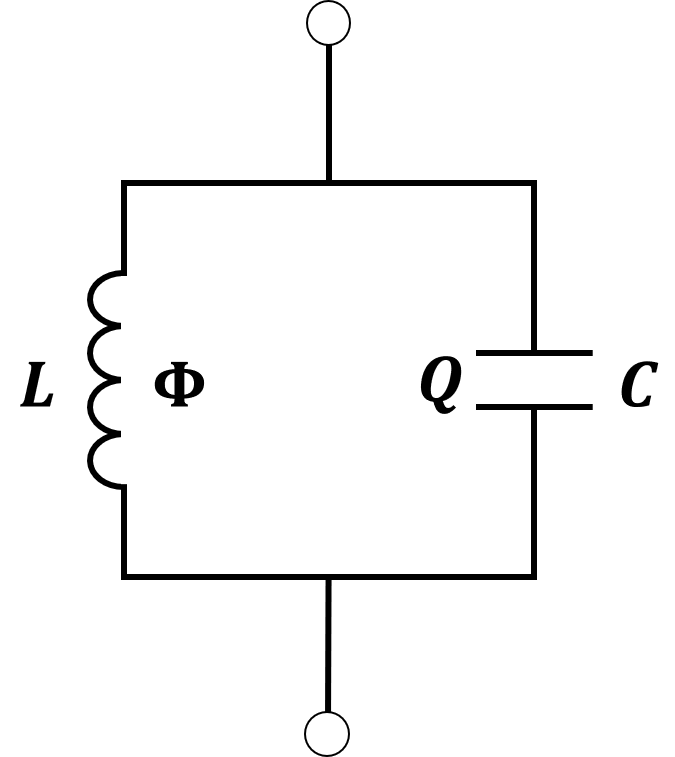
\includegraphics[width=4cm]{LCResonator.png}
                \caption{LC共振器}
            \end{center}
        \end{figure}
        一般化座標として磁束$\Phi$を用いることとすると、Faradayの法則及びインダクタンス$L$の定義式から
        \begin{eqnarray}
            V&=&\frac{d\Phi}{dt}=\dot{\Phi},\\
            \Phi&=&-LI
        \end{eqnarray}
        が導かれる。回路の運動エネルギー$T$及びポテンシャルエネルギー$U$は、
        \begin{eqnarray}
            T=C\int V dV & = & \frac{1}{2}C \dot{\Phi}^2,\\
            U=L\int I dI & = & \frac{1}{2L} \Phi^2
        \end{eqnarray}
        で与えられ、これよりLagrangian\quad$\mathcal{L}$は
        \begin{equation}
            \mathcal{L}(\Phi,\dot{\Phi})=T-U=\frac{1}{2}C \dot{\Phi}^2-\frac{1}{2L} \Phi^2
        \end{equation}
        と記述される。したがって一般化運動量$Q$は
        \begin{equation}
            Q = \frac{\partial\mathcal{L}}{\partial \dot{\Phi}}=C\dot{\Phi}
        \end{equation}
        となる。HamiltonianはLagrangianをLegendre変換して
        \begin{equation}
            \mathcal{H}(\Phi,Q)=Q\dot{\Phi}-\mathcal{L}=\frac{1}{2C}Q^2+\frac{1}{2L}\Phi^2
        \end{equation}
        と求まる。
        ()式は()式において
        \begin{equation}
        \begin{split}
             q \to Q,\; &p \to -\Phi,\\
             m\omega^2 \to \frac{1}{C},\; m \to &L, \; \omega \to \frac{1}{\sqrt{LC}}
        \end{split}
        \end{equation}
        と置き換えたものと等価であり、調和振動子の場合と同様にこの系も量子化が可能である。正準変数$\hat{Q},\hat{\Phi}$と昇降演算子$\hat{a},\hat{a}^\dagger$は
        \begin{eqnarray}
            \hat{Q}=\sqrt{\frac{\hbar}{2}\omega C}(\hat{a}+\hat{a}^\dagger)\\
            \hat{\Phi}=i\sqrt{\frac{\hbar}{2}\frac{1}{\omega C}}(\hat{a}-\hat{a}^\dagger)
        \end{eqnarray}
        という関係式で結ばれ、最終的には定数項を落とすことでHamiltonianを()式同様
        \begin{equation}
            \mathcal{H}=\hbar\omega\hat{a}^\dagger\hat{a}
        \end{equation}
        の形に書くことができる。
        \subsection{ジョセフソン接合}
        2つの超伝導体の間に絶縁体もしくは常伝導体などの極めて薄い障壁をさしはさむことにより、2つの超伝導体間には超伝導電流が流れる。
        1962年にB. D. Josephsonによって発見されたこの効果をジョセフソン効果、超伝導体-障壁-超伝導体の接合をジョセフソン接合という。\\

        \begin{figure}[H]
            \begin{center}
                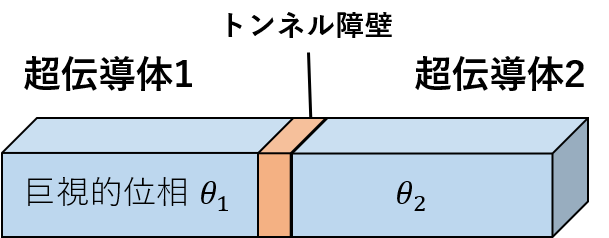
\includegraphics[width=7cm]{JJ.png}
                \caption{ジョセフソン接合}
            \end{center}
        \end{figure}

        金属が超伝導体となるとき、すべての電子が同じふるまいをする巨視的量子状態が出現し、電子の波動関数は粒子数$N$と巨視的位相$\theta$によって記述される。
        超伝導体1,2の巨視的位相をそれぞれ$\theta_1,\theta_2$とすると、流れる電流$I$は位相差$\varphi=\theta_1-\theta_2$を用いて
        \begin{equation}
            I=I_c \sin\varphi
        \end{equation}
        という式で表される(直流ジョセフソン効果)。ここで、$I_c$はジョセフソン接合を流れる最大の電流であり、臨界電流と呼ばれる。
        $I_c$はAmbegaokar=Baratoffの式より以下のように求められ
        \begin{equation}
            I_c=\frac{\pi \Delta(T)}{2eR_n}\tanh(\frac{\Delta(T)}{2k_BT})
        \end{equation}
        \begin{equation*}
            T:\mathrm{絶対温度},\quad \Delta(T):超伝導体のバンドギャップ,\quad R_n:障壁の抵抗
        \end{equation*}
        温度依存性を有するが、実験での量子ビット系は$T \sim 10$mKの温度領域におかれるため上式は
        \begin{equation}
            I_c=\frac{\pi \Delta(0)}{2eR_n}
        \end{equation}
        と近似できる。式(),()から分かるように、流れる臨界電流は超伝導体間の電位差に関係なく、位相差のみによって決定される。\\
        ジョセフソン接合における電位Vと位相差$\varphi$の間には以下の関係があり、
        \begin{equation}
            \frac{\partial\varphi}{\partial t}=\frac{2e}{\hbar}V
        \end{equation}
        で表せることが知られている(交流ジョセフソン効果)。()式、()式を用いると、ジョセフソン接合が持つポテンシャルエネルギーは
        \begin{equation}
        \begin{split}
            U&=\int IVdt \\
            &= \frac{\hbar I_c}{2e}\int \sin \varphi \frac{d\varphi}{dt}dt \\
            &= -E_J \cos \varphi
        \end{split}
        \end{equation}
        となり、非線形な項で表されることになる。ここで、
        \begin{equation}
            E_J=\frac{\hbar I_c}{2e}
        \end{equation}
        はジョセフソンエネルギーと呼ばれる量である。\\
        ジョセフソン接合の回路記号を以下図()のように表す。なお実際のジョセフソン接合には()式中の障壁の抵抗$R_n$の他にキャパシタンス$C_J$が存在し、
        図()のように接合に並列に含まれていると考える。
        \begin{figure}[htbp]
            \begin{center}
                \begin{tabular}{c}
                    \begin{minipage}{0.5\hsize}
                        \begin{center}
                            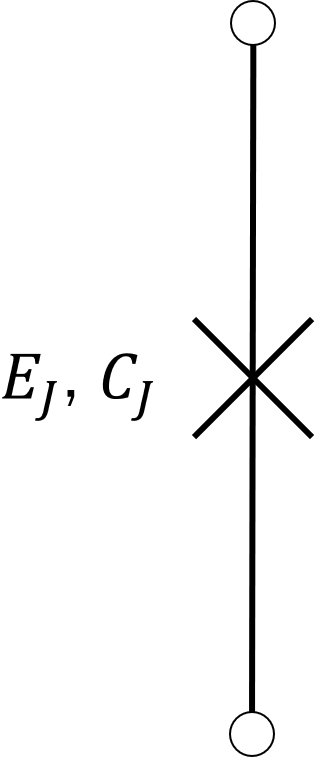
\includegraphics[width=1.5cm]{Joseph.png}
                        \end{center}
                        \captionsetup{labelformat=empty,labelsep=none}
                        \caption{[a]}
                    \end{minipage}
                    
                    \begin{minipage}{0.5\hsize}
                        \begin{center}
                            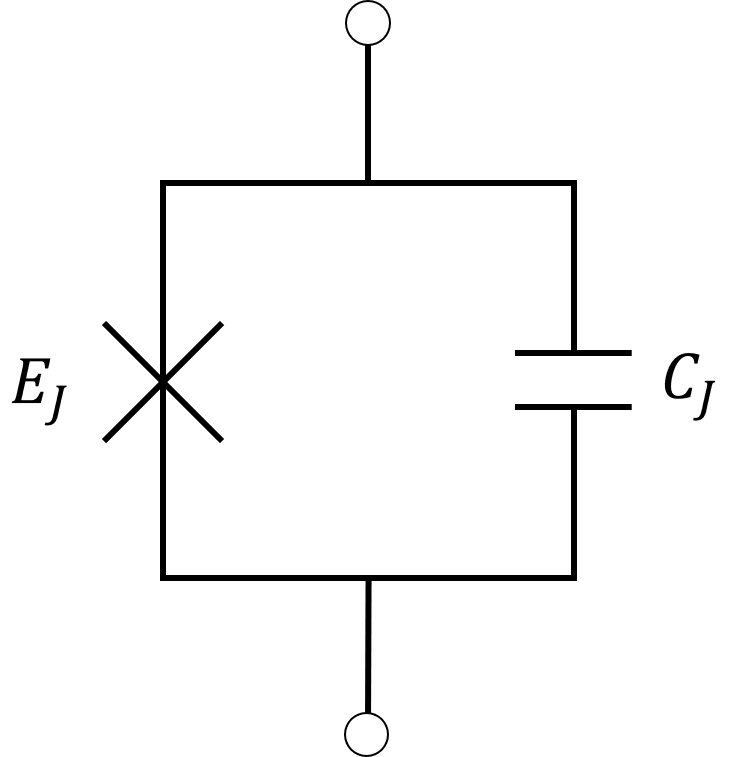
\includegraphics[width=3cm]{Joseph_real.png}
                        \end{center}
                        \captionsetup{labelformat=empty,labelsep=none}
                        \caption{[b]}
                    \end{minipage}
                \end{tabular}
                \caption{ジョセフソン接合の回路記号}
            \end{center}
        \end{figure}
        \subsubsection{DC-SQUID}
        次に、ジョセフソン接合を利用した素子であるSQUID(Superconducting quantum interference device) について説明する。
        DC-SQUIDは図()のような、ジョセフソン接合が2つ挿入された超伝導体ループから形成される。
        \begin{figure}
            \begin{center}
                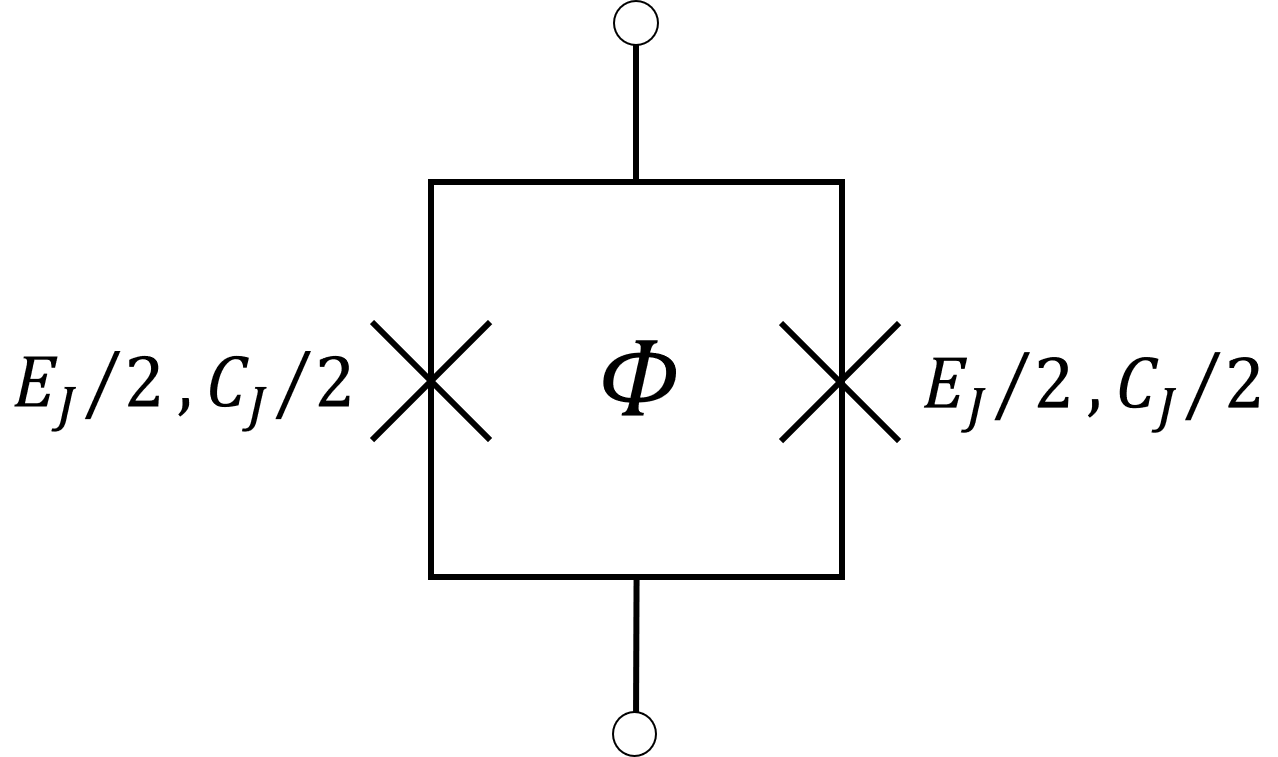
\includegraphics[width=5cm]{DCsquid.png}
                \caption{DC-SQUID}
            \end{center}
        \end{figure}
        Josephson接合のときと同様、ポテンシャルエネルギーを計算すると
        \begin{equation}
        \begin{split}
             U&=-\frac{E_J}{2} \cos \varphi_1-\frac{E_J}{2} \cos \varphi_2\\
            &=-E_J \cos (\frac{\varphi_1+\varphi_2}{2})\cos (\frac{\varphi_1-\varphi_2}{2})
        \end{split} 
        \end{equation}
        となる。ここで、超伝導ループにおける磁束の量子化の条件より
        \begin{equation}
        \begin{split}
            \frac{2\pi \Phi}{\Phi_0}+\varphi_1-\varphi_2=0 , \;  \Phi_0 = 2\pi\frac{\hbar}{2e}\\
            \Phi_0 : \mathrm{磁束量子(flux quanta)}
        \end{split}    
        \end{equation}
        を利用し、()式は
        \begin{equation}
            U=-E_J \cos (\frac{\varphi_1+\varphi_2}{2})\cos (\pi\frac{\Phi}{\Phi_0})
        \end{equation}
        と書き換えられる。()式と比較すると、
        \begin{equation}
            E_J \to E_J \cos (\pi\frac{\Phi}{\Phi_0}) , \;\varphi \to \frac{\varphi_1+\varphi_2}{2}
        \end{equation}
        という対応関係があることが分かる。これによってSQUIDは外部からの磁束$\Phi$によってジョセフソンエネルギーを変化させられる
        ジョセフソン接合として扱うことができる。
        \subsection{SQUIDによる量子ビットの実装}
        ジョセフソン接合によりポテンシャルエネルギーに非線形性を持たせ、なおかつSQUIDの導入によりそれを外部磁束で制御できるようになることを示した。
        ここからはLC共振器とSQUIDによって量子ビットを実装する方法について説明する。
        図()のようにキャパシタンス$C_g$を介してジョセフソン接合に電圧$V_g$がかかっている系を考える。
        \begin{figure}[H]
            \begin{center}
                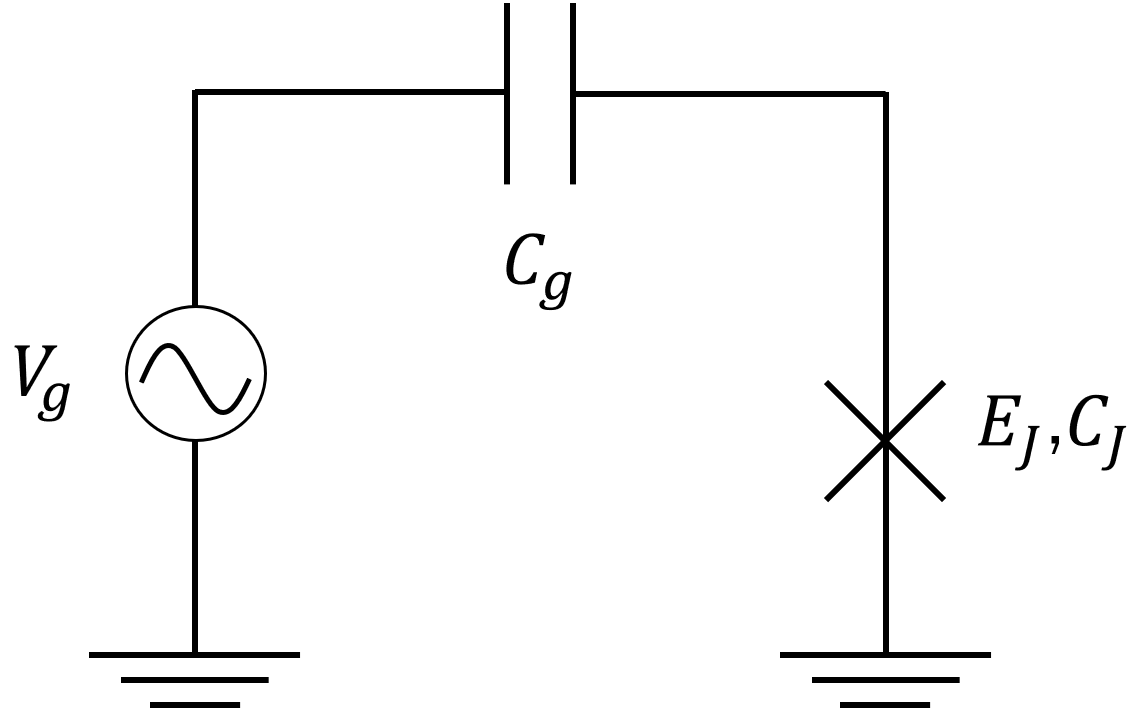
\includegraphics[width=5cm]{CPB.png}
                \caption{クーパー対箱}
            \end{center}
        \end{figure}
        運動エネルギーT,ポテンシャルエネルギーUは磁束$\Phi$を一般化座標として
        \begin{eqnarray}
            T=\frac{1}{2}C_J\dot{\Phi}^2+\frac{1}{2}C_g(\dot{\Phi}-V_g)^2\\
            U=-E_J\cos(\phi)
        \end{eqnarray}
        となる。ここでジョセフソン接合における位相差$\phi$はジョセフソン効果の式から磁束$\Phi$と
        \begin{equation}
            \dot{\Phi}=\frac{\hbar}{2e}\dot{\phi}
        \end{equation}
        という関係を持つ。
        一般化座標を$\phi$におきかえるとLagrangianは
        \begin{equation}
            \frac{1}{2}\left(\frac{\hbar}{2 e}\right)^{2} C_{J} \dot{\phi}^{2}+\frac{1}{2} C_{g}\left(\frac{\hbar}{2 e} \dot{\phi}-V_{g}\right)^{2}+E_{J} \cos \phi
        \end{equation}
        となり、位相差$\phi$に共役な変数$q$は
        \begin{equation}
            q=\frac{\partial \mathcal{L}}{\partial \dot{\phi}}=\left(\frac{\hbar}{2 e}\right)^{2} C_{J} \dot{\phi}+\frac{\hbar}{2 e} C_{g}\left(\frac{\hbar}{2 e} \dot{\phi}-V_{g}\right)=\frac{\hbar}{2 e} Q
        \end{equation}
        という関係にある。以上よりLegendre変換を用いてHamiltonianは
        \begin{equation}
        \begin{split}
            \mathcal{H}(\phi, q)
            &=q \dot{\phi}-\mathcal{L}\\
            &=\frac{1}{2}\left(\frac{\hbar}{2 e}\right)C_{J} \dot{\phi}^{2}+\frac{1}{2}\left(\frac{\hbar}{2 e}\right)^{2} C_{g} \dot{\phi}^{2}-\frac{1}{2} C_{g} V_{g}^{2}-E_{J} \cos \phi
        \end{split}
        \end{equation}
        と求められる。\\
        超伝導体内における電荷は、2つの電子が電子-格子相互作用によって対をなしたCooper対と呼ばれるものであり
        超伝導体の電荷数$n$を
        \begin{equation}n=\frac{Q}{2 e}=\frac{q}{\hbar}\end{equation}
        と定める。またゲート電圧$V_g$が掛かっている部分の電荷数について
        \begin{equation}n_{g}=-\frac{C_{g} V_{g}}{2 e}\end{equation}
        と定めれば
        \begin{equation}\mathcal{H}(\phi, q)=\frac{(2 e)^{2}}{2\left(C_{J}+C_{g}\right)}\left(n-n_{g}\right)^{2}-\frac{(2 e)^{2}}{2 C_{g}} n_g^{2}-E_{J} \cos \phi\end{equation}
        と書ける。ここで量子ビットの帯電エネルギー、すなわちジョセフソン帯電エネルギーを
        \begin{equation}E_{C}=\frac{e^{2}}{2 C_{\Sigma}}, \quad C_{\Sigma}=C_{J}+C_{g}\end{equation}
        で定義する。以上により定数項を落としたハミルトニアンは
        \begin{equation}\mathcal{H}=4 E_{C}\left(n-n_{g}\right)^{2}-E_{J} \cos \phi\end{equation}
        のように記述される。\\
        このHamiltonianの量子化のため、正準変数$\phi,q$に対し交換関係
        \begin{equation}[\hat{\phi}, \hat{q}]=i \hbar\end{equation}
        を導入する。ここで$\hat{n}=\hat{q} / \hbar$であるため
        \begin{equation}[\hat{\phi}, \hat{n}]=\frac{1}{\hbar}[\hat{\phi}, \hat{q}]=i\end{equation}
        が成立する。電荷数$\hat{n}$はエルミート演算子であるため固有状態$\ket{n}$と固有値$n$を用いて
        \begin{equation}\hat{n}=\sum_{n} n|n\rangle\langle n|\end{equation}
        と書くことができる。
        このとき$e^{\pm i \hat{\phi}}$は昇降演算子となることが知られており
        \begin{equation}e^{i \hat{\phi}}=\sum_{n}\ket{n+1}\bra{n}, \quad e^{-i \hat{\phi}}=\sum_{n}\ket{n}\bra{n+1}\end{equation}
        と書ける。これにより
        \begin{equation}
            \cos \hat{\phi} = \frac{1}{2}(e^{i \hat{\phi}}+e^{-i \hat{\phi}})=\frac{1}{2}\sum_{n}(\ket{n+1}\bra{n}+\ket{n}\bra{n+1})
        \end{equation}
        となるので電荷量子ビットのHamiltonianは
        \begin{equation}\begin{aligned}
            \hat{\mathcal{H}} &=4 E_{C}\left(\hat{n}-n_{g}\right)^{2}-E_{J} \cos \hat{\phi} \\
            &=4 E_{C} \sum_{n}\left(n-n_{g}\right)^{2}\ket{n}\bra{n}-\frac{E_{J}}{2} \sum_{n}(\ket{n+1}\bra{n}+\ket{n}\bra{n+1})
            \end{aligned}\end{equation}
        となる。
    \subsection{他素子との結合}
        \subsubsection{共振器との結合}
        \subsubsection{量子ビットとの結合}
    \subsection{デコヒーレンス}
        \subsubsection{$T_1$,$T_2$,$T_2^E$}

\section{量子ビットゲート}
    \subsection{1qubitゲート}
        \subsubsection{X,Y軸回転}
        \subsubsection{Z軸回転}
        \subsubsection{その他の重要1qubitゲート}
    \subsection{CZゲート}
        \subsubsection{CZゲートの理論}
        \subsubsection{実装上の課題1.CZゲートの断熱・非断熱過程}
        \subsubsection{実装上の課題2.低周波磁束ノイズ}
        \subsubsection{パルス制御}

        
        

\chapter{波形のシミュレーション}
    \begin{abstract}
    \end{abstract}
    \section{Net-Zero Pulseの最適化シミュレーション}
前章で説明したああああ


\chapter{サンプル作製}
    \begin{abstract}
    \end{abstract}
    \section{Overview}
    今回測定したサンプルは2章で述べた量子ビット-量子ビット直接結合系を作ることを想定して作製した。
    図()にサンプル(チップのみ)の全体図を示す。
    \begin{figure}[H]
        \begin{center}
            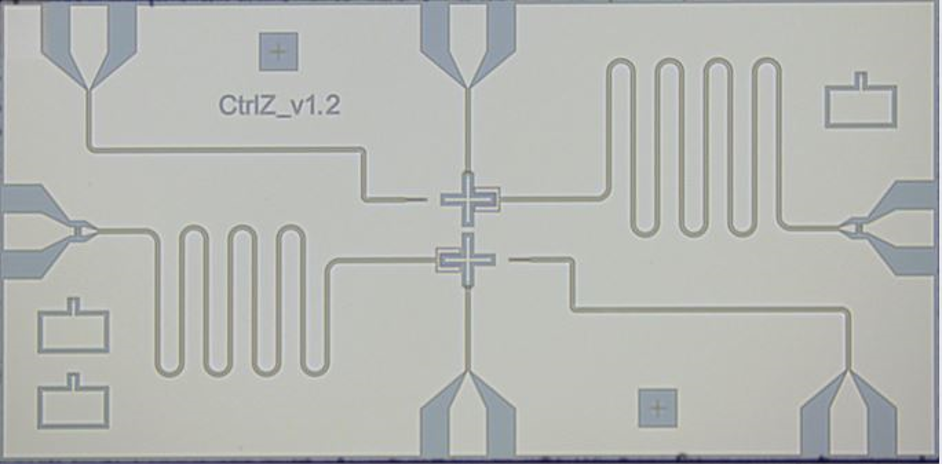
\includegraphics[width=12cm]{Chippic.png}
            \caption{作製したサンプル}
        \end{center}
    \end{figure}
    本サンプルは厚さ450umのシリコン基板に厚さ50nmのNbをスパッタした縦2.5$\times$横5mmのチップに加工を施し作製した。
    図の中央にある2つの十字はTunableなTransmon型量子ビットである。この形のTransmonは別名Xmon\cite{barends2013coherent}とも呼ばれ、
    周囲のコンポーネントとの配線のしやすさ、コヒーレンス時間の長さから電荷量子ビットベースの量子コンピュータで主流の形状である。\footnote{他にも繋げられる配線数を重視したTransmonとして多脚のStarmon,円形のConcentric Qubitなどのデザインも研究されている}
    量子ビット同士はキャパシティブに結合されている。量子ビットにつながる配線のうち、蛇行している配線はCPW(後述)である。図の垂直方向にXmonに向かって配線されているラインは量子ビットに磁束バイアスを与えるためのバイアスラインである。この図では見えづらいが、量子ビットのバイアスライン側にはAl-AlOx-AlからなるSQUIDがついており、バイアスラインから流す直流電流でSQUID内の磁束を調整する。
    チップ左上および右下から伸びている配線は1qubit回転ゲートのためのマイクロ波をXmonに送り込むコントロールラインとなっている。
    その他左下、右上に配置された凸型の素子は各々の量子ビットのテスト用ジャンクションであり、バイアスラインのポートとコントロールラインのポート間にあるのはアライメントマークである。
\subsubsection{CPW}
CPW (Coplanar Waveguide,コプレーナ共振器) は図のような構造をした共振器である。
\begin{figure}[H]
    \begin{center}
        \includegraphics[width=10cm]{CPW_img.png}
        \caption{CPWの構造}
    \end{center}
\end{figure}
比誘電率$\epsilon_r$の基板上には接地導体を挟んで中央に導体の線路が通っている。
共振周波数は光速$c$,電磁波の伝播方向への長さ$l$,そして基板及び上部の空間の形状から決定される実効的な比誘電率$\epsilon_{eff}$を用いて
\begin{equation}
    \omega_{r}=\frac{c \pi}{l \sqrt{\epsilon_{e f f}}}
\end{equation}
で与えられる。\\ %ここで実効的な比誘電率の値には$\epsilon_{e f f}=6.33$を用いた。
共振器全体のQ値($Q_{load}$は、外部素子との結合に由来する外部Q値($Q_{ext}$)及び共振器そのものの品質による内部Q値$Q_{int}$の成分に分けられ
\begin{equation}
    \frac{1}{Q_{l}}=\frac{1}{Q_{int}}+\frac{1}{Q_{ext}}
\end{equation}
という関係がある。このうち内部Q値に関しては共振器の材質や作製プロセスに大きく依存するので、外部のコンポーネントとの結合をキャパシタンスなどで調整して全体のQ値を変えることになる。

\section{設計値・留意した点}
作製したサンプルの等価回路モデル図を図()に示す。
\begin{figure}[H]
    \begin{center}
        \includegraphics[width=14cm]{Circdiagram.png}
        \caption{作製したサンプルの等価回路図}
    \end{center}
\end{figure}
図()の各種コンポーネントの周波数、キャパシタンス等の値の決定にあたっては、状態操作及び読み出しを適切に行うために、いくつかの制約が存在する。
\subsection{共振器の設計}
まず共振器については、我々の研究室が所有するローパスフィルタが$4 \sim 8$GHz,$8 \sim 12$GHzのレンジにあるため
4または8GHzの上下にまたがる周波数は避けるべきである。また共振器の周波数が低すぎると()式から共振器長を延長しなければならず
チップの限られたスペースを圧迫するため好ましくない。分散読み出しの条件$(\Delta = |\omega_r − \omega_q|\gg g)$を達成するために共振器と量子ビットの周波数を1GHz程離す必要があり、結合定数$g_{01}$も大きくて100MHz台に抑制される。
最後に、共振器からの光子放出レート$\kappa$について、これが弱結合領域($\kappa<g_{01},\Gamma_1$)の範囲に来るように設定した。この領域では状態読み出しが遅くなるものの
量子ビットのエネルギー緩和を低くとどめられる。
これらのことを考慮した上でシミュレーションを通じて共振器に関係するパラメータを以下のように定めた。
値の見積もりに際しては
\begin{table}[H]
    \begin{center}
    \begin{tabular}{c}
        \begin{minipage}{0.45\hsize}
            \begin{center}
                \begin{tabular}{|c|c|}
                    \hline
                    & [GHz] \\
                    \hline
                    \hline
                        共振器1の周波数$f_{r1}$ & 6.5 \\
                    \hline
                        共振器1の光子放出レート$\kappa_1$ & 2.3 [MHz]
                    \hline
                        共振器2の周波数$f_{r2}$ & 7.4 \\
                    \hline
                        共振器2の光子放出レート$\kappa_2$ & 1.6 [MHz]
                    \hline
                        量子ビット1と共振器1の結合定数$g^{01}$ & 0.068\\
                    \hline
                        量子ビット2と共振器2の結合定数$g^{01}$ & 0.073 \\
                    \hline
                \end{tabular}
            \end{center}
        \end{minipage}

        \begin{minipage}{0.4\hsize}
            \begin{center}
              \begin{tabular}{|c|c|}
                \hline
                \hline
                 & [fF]\\ 
                \hline 
                \hline
                $f_{r1}$ &  6.8\\
                $f_{r2}$ &  6.0\\
                $C_{in,1}$ &  8.0\\
                $C_{in,2}$ &  7.1\\
                \hline
              \end{tabular}
            \end{center}
          \end{minipage}
          \caption{共振器関係のパラメータ}
        \end{tabular}
    \end{center}
\end{table}
\subsection{量子ビットの設計}
量子ビットの固有周波数$\omega_q$は,$E_J,E_C$を用いて以下のように表される。
\begin{equation}
    \omega_q = \sqrt{8E_JE_C}-E_C \\
\end{equation}
このとき
\begin{equation}
    \begin{aligned}
        E_C &= \frac{e^2}{2C_{\Sigma}}\\
        C_{\Sigma} & = C_B+C_g+C_J\\
        E_J &= E_{J,max}|\cos(\pi \Phi/\Phi_0)| \\
        E_{J,max} &= \frac{I_C}{2e} \\
        I_C &= J_{C}A\\
        J_{C}&=\frac{\pi \Delta(T)}{2 e R_{n} A} \tanh \left(\frac{\Delta(T)}{2 k_{B} T}\right)
    \end{aligned}
\end{equation}
量子ビット間の結合定数$J$は結合部のキャパシタンス$C_c$を用いて
\begin{equation}
    J=C_{c} \approx \frac{1}{2} \frac{C_{c}}{\sqrt{C_{\Sigma}^{(1)} C_{\Sigma}^{(2)}}} \sqrt{\omega_{\mathrm{q}}^{(1)} \omega_{\mathrm{q}}^{(2)}}
\end{equation}
として見積もった。\\
ジョセフソン接合のキャパシタンス$C_J$については自分で設計できる量ではないので2~3fF程度として計算した。
2量子ビット直接結合系の場合、量子ビット同士の周波数が近すぎると一方のビットに送られたマイクロ波で他方のビットが状態操作される可能性があるため\footnote{原理の章での説明を省いたが、この作用を積極的に利用する、CR(Cross-Resonance)ゲートと呼ばれる2量子ビットゲートも存在する。CRゲートは特定のゲート時間だけ一方の量子ビットを他方の量子ビットの共振周波数のマイクロ波で駆動することにより、CNOTのユニタリ演算を実現できる。}
そのため、設計の上では量子ビットの周波数を800MHzほど離調している。量子ビット同士の結合定数$J$は強くなるほど式()よりゲート時間が短くなるが
状態操作を行わない状態での量子ビット間のエネルギー交換も行われやすくなるため大きくても20MHz台に設計する。\\
\begin{table}[H]
    \begin{center}
    \begin{tabular}{c}
        \begin{minipage}{0.45\hsize}
            \begin{center}
                \caption{量子ビット1,2の周波数単位のパラメータ}
                \begin{tabular}{|c|c|}
                    \hline
                    & [GHz] \\
                    \hline
                    \hline
                        量子ビット1の周波数$\omega_{q1}$ & 5.78 \\
                    \hline
                        〃非調和性$\alpha_{1}$ & -0.304\\
                    \hline
                        量子ビット2の周波数$\omega_{q2}$ & 6.61 \\
                    \hline
                        〃非調和性$\alpha_{1}$ & -0.298 \\
                    \hline
                        $E_{C1}$ & 0.27 \\
                    \hline
                        $E_{J1}$ & 17 \\
                    \hline
                        $E_{C2}$ & 0.27 \\
                    \hline
                        $E_{J2}$ & 22 \\
                    \hline
                        結合定数$J$ & 0.015\\
                    \hline
                \end{tabular}
            \end{center}
        \end{minipage}

        \begin{minipage}{0.4\hsize}
            \begin{center}
              \caption{キャパシタンスのシミュレート結果}
              \begin{tabular}{|c|c|}
                \hline
                \hline
                 & [fF]\\ 
                \hline 
                \hline
                $C_{B1}$ & 71.745 \\
                $C_{B2}$ & 71.745\\
                $C_{g1}$ &  6.8\\
                $C_{g2}$ &  6.0\\
                \hline
              \end{tabular}
            \end{center}
          \end{minipage}
        \end{tabular}
    \end{center}
\end{table}
\section{電磁界シミュレーション}共振器の周波数、各種キャパシタンスはCAD上で図面を設計し、AWR Micrwave officeというソフトウェアを用いてシミュレートした。
Microwave officeでは2次元図面に厚みを設定して誘電体と金属の層に対する設定を行うことで3次元に近い状況でのシミュレーションを行う。
また、超伝導体については電気抵抗がほぼない導体(電気伝導度=$10^{200}$)に近似した。\\
\begin{figure}[H]
    \begin{center}
        \includegraphics[width=14cm]{keisokutyuu.PNG}
        \caption{Microwave officeに取り込んだサンプル図面。共振器2の周波数特性をシミュレート中}
    \end{center}
\end{figure}
\begin{figure}[H]
    \begin{center}
        \begin{tabular}{c}
            \begin{minipage}{0.5\hsize}
                \begin{center}
                    \includegraphics[width=6cm]{Interdigitalcap.PNG}
                \end{center}
                %\captionsetup{labelformat=empty,labelsep=none}
                \caption{Interdigital capacitor}
            \end{minipage}
            
            \begin{minipage}{0.5\hsize}
                \begin{center}
                    \includegraphics[width=6cm]{keisokutyuu_bias.PNG}
                \end{center}
                %\captionsetup{labelformat=empty,labelsep=none}
                \caption{量子ビット付近拡大}
            \end{minipage}
        \end{tabular}
    \end{center}
\end{figure}
読み出しポート近くを拡大すると、Interdigital capacitorが配置されており、この形状の微調整により$C_in$の大きさを調節した。
またバイアスライン付近は図()のようになっているが、Microwave officeはインダクタンスを含めたシミュレーションはできないのでこの時点でSQUIDループは解析に加えていない。
まず共振器については図()のようにポートを配置し、ポート1からグラウンドポート-1に向けて送信するマイクロ波の反射係数S11を見ることで周波数特性を解析した。
量子ビット1,2にそれぞれ接続された共振器R1,R2の周波数特性は図()のとおりである。最終的にはこの曲線をResonator-tools \url{https://github.com/sebastianprobst/resonator_tools}を用いてfittingし
$Q_{in},Q_{out},\kappa$を求めた。
\begin{figure}[H]
    \begin{center}
        \includegraphics[width=10cm]{R1R2freq.png}
        \caption{共振器1,2の共振周波数}
    \end{center}
\end{figure}
また、ポート間のアドミタンス$Y$の周波数特性を見ることでコンポーネント間のキャパシタンスを見積もることもできる。インピーダンスを$Z$とすると
\begin{equation}
\begin{aligned}
    Z = R + j\omega L + \frac{1}{j\omega C} \\
    Y = 1/Z
\end{aligned}
\end{equation}
であり、超伝導体では$R \to 0$となる。さらに$\omega$が小さい領域では$L$を含む項の寄与は無視できるため
\begin{equation}
        Y \sim j\omega C
\end{equation}
と表現される。アドミタンスの虚部を$f$に対してプロットすると傾き$2\pi C$が得られ、ここからCの値が得られる。
(Im[Y]を測る周波数領域は$f=0 \sim 1.0$GHzまでとした。)
\section{作製手順}
チップの作製にあたっては理化学研究所内クリーンルームにてパッケージングを除く全作業を行った。このうちの大まかな工程について述べる。
\subsubsection{1.Photolithography}
デザインにおけるジョセフソン接合以外の部分(共振器,量子ビット本体)をチップ上にパターニングする工程。
ここでは2×2cmのチップに2.5×5mmのデザインを8×4個配置したパターンを一遍に描画した。
レジストとしてZEP520A-7をスピンコーターを用いて塗布し、マスクレスUV露光装置を用いてUVを照射。
現像後、CF4ガスによるエッチングを施し、残留レジストを剥離液で洗い流す。
\subsubsection{2.EBL}
続いて電子ビーム描画装置によりジョセフソン接合部分のパターンを描画した。
先ほどのUVを照射するPhotolithographyと比較してビーム径が小さいので、より精緻なデザインを描画できる。
2層のレジストZEP520A-7, Copolymerを塗布しホットプレートで焼き固め、ビーム照射後に上層のZEPのみを現像した。
その後IPA(イソプロピルアルコール)と超純水93:7溶液でZEPに穴が空いた箇所のCopolymerを現像した。
ここまでの作業によりSQUID付近には図()に示す、ジョセフソン接合を蒸着するための空洞が形成される。
\subsubsection{3.PLASSYS}
\begin{figure}[H]
    \begin{center}
        \includegraphics[width=16cm]{PLASSYS_stage0.png}
        \caption{EBL終了後のレジストによる空洞}
    \end{center}
\end{figure}
\begin{figure}[H]
    \begin{center}
        \includegraphics[width=16cm]{PLASSYS_stage1.png}
        \caption{2角度蒸着法:一回目のアルミ蒸着後}
    \end{center}
\end{figure}
\begin{figure}[H]
    \begin{center}
        \includegraphics[width=16cm]{PLASSYS_stage2.png}
        \caption{アルミの酸化被膜形成}
    \end{center}
\end{figure}
\begin{figure}[H]
    \begin{center}
        \includegraphics[width=8cm]{JJ_img_zoomup.png}
        \caption{ジョセフソン接合,重なり部分}
    \end{center}
\end{figure}
ジョセフソン接合はAl-AlOx-Alの重なりを作るために2角度蒸着法という工程によって形成される。
最初に少し角度$\theta$をつけた状態で一層目のアルミが蒸着され、10分程O2ガスによって酸化されたのち
二層目のアルミが先ほどとは逆向きに同じ角度で蒸着される。一層目の酸化被膜がジョセフソン接合の薄膜障壁の役割を果たし、
この被膜と2層目のアルミの重なり面積によりここを通るジョセフソン電流の臨界電流値が決定される。
重なり面積$S$は図中に示すパラメータを用いて
\begin{equation}
    S = (2y \tan \theta -g)R
\end{equation}
と求められ、電流密度Jが既知であれば式(),()により$I_{J,max}$が求められる。
自身のサンプルで設計に用いた値を表()に示す。
\begin{table}[H]
    \caption{ジョセフソン接合作製時のパラメータ}
    \begin{center}
    \begin{tabular}{|c|c|}
    \hline
     & [nm]\\
    \hline
    \hline
    x & 300\\
    \hline
    y & 600\\
    \hline
    R & Q1側:250, Q2側:320\\
    \hline
    w & 350 \\
    \hline
    g & 295 \\
    \hline
    \end{tabular}
\end{center}
\end{table}
蒸着後、接合部ではない箇所のアルミを剥離液で剥がし、SEM(走査電子顕微鏡)によりジャンクションが形成されていることを確認した。
SEMによるジャンクション付近の撮影の結果を図()に示す。
\begin{figure}[H]
    \begin{center}
        \begin{tabular}{c}
            \begin{minipage}{0.5\hsize}
                \begin{center}
                    \includegraphics[width=6cm]{Ino_test_up.jpg}
                \end{center}
                %\captionsetup{labelformat=empty,labelsep=none}
                \caption{2角度蒸着法で形成されたジョセフソン接合}
            \end{minipage}
            
            \begin{minipage}{0.5\hsize}
                \begin{center}
                    \includegraphics[width=6cm]{Ino_test_upL.jpg}
                \end{center}
                %\captionsetup{labelformat=empty,labelsep=none}
                \caption{接合部の拡大図}
            \end{minipage}
        \end{tabular}
    \end{center}
\end{figure}
\subsubsection{4.Dicing}
UVレジストを塗布・焼き固めたのち、チップを2.5×5mmに切り出す。アセトンとIPAでレジスト剥離、洗浄を行いチップが完成する。
\subsection{パッケージング}
完成したサンプルは専用のサンプルホルダー(図())に装着される。
\begin{figure}[H]
    \begin{center}
        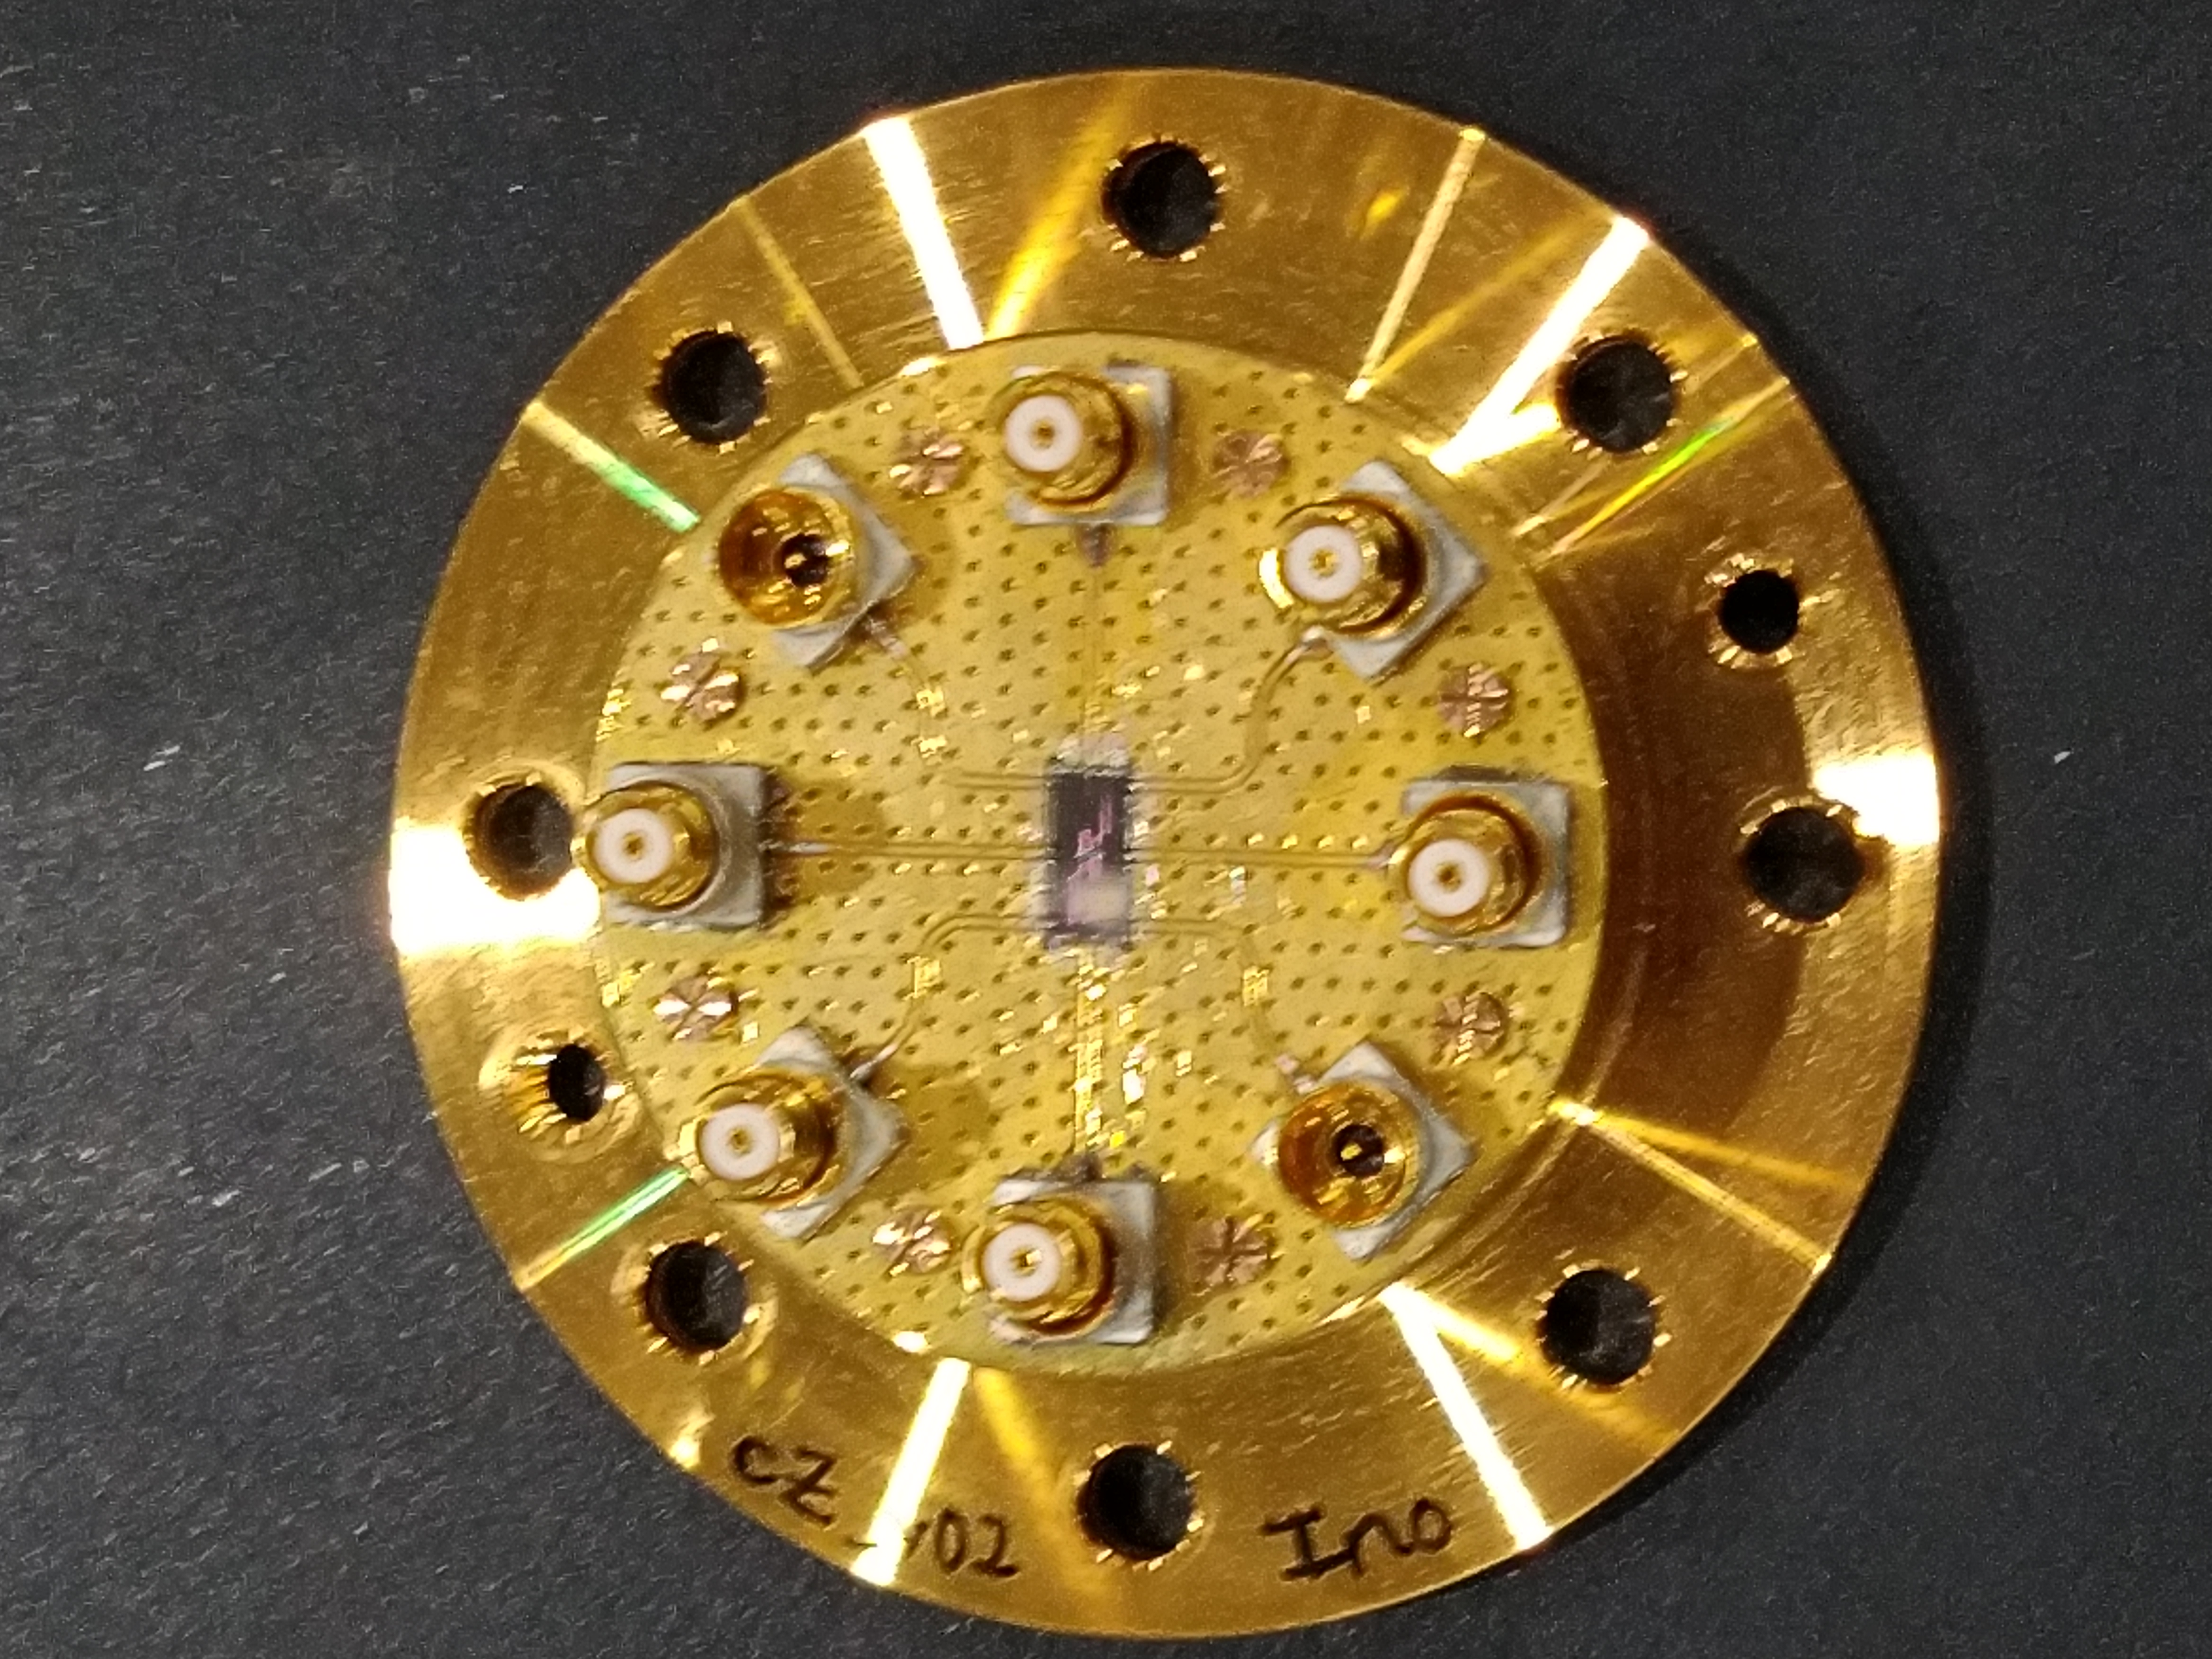
\includegraphics[width=7cm,angle=-90]{sample_from_above.jpg}
        \caption{サンプルホルダーに装着されたチップ}
    \end{center}
\end{figure}
サンプルホルダー上面はPCB(Printed Circuit Board,プリント基板)となっており
チップの固定ならびに接続されたSMAコネクタ経由で送られてくる信号をチップ上のポートに伝送する役割を担う。
\begin{figure}[H]
    \begin{center}
        \begin{tabular}{c}
            \begin{minipage}{0.5\hsize}
                \begin{center}
                    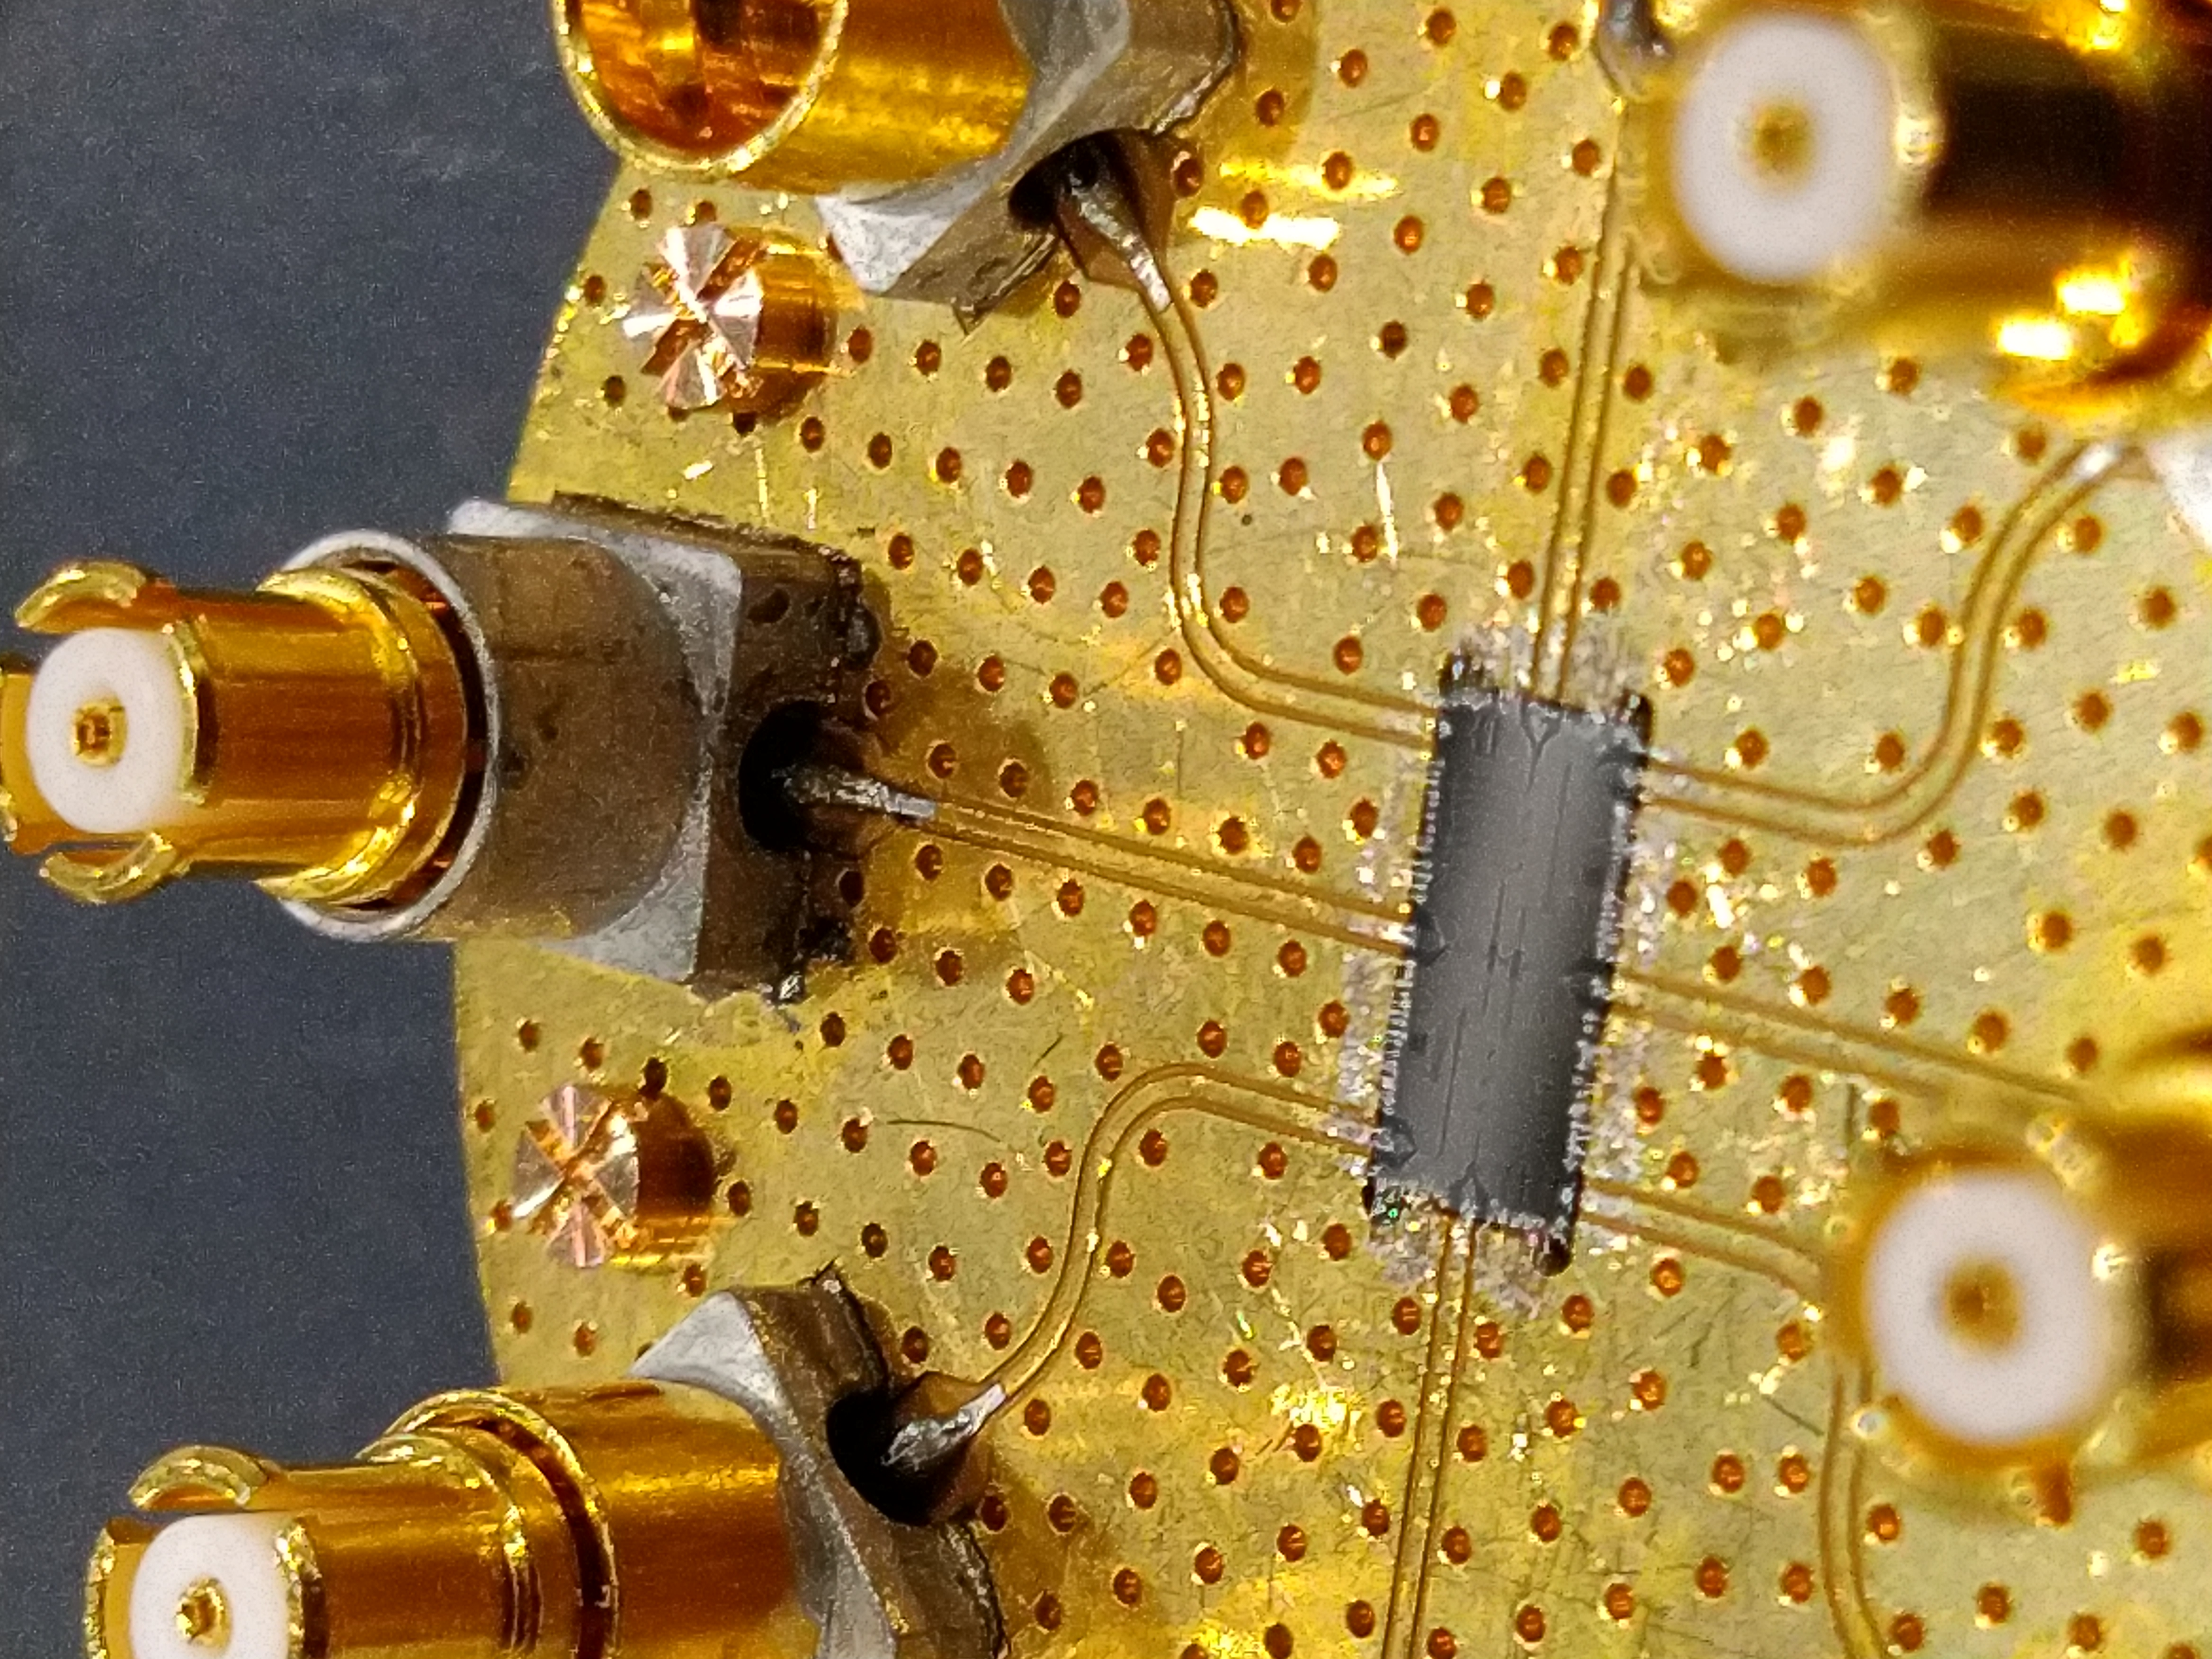
\includegraphics[width=6cm,angle=-90]{zoomup_SMA_PCB.jpg}
                \end{center}
                %\captionsetup{labelformat=empty,labelsep=none}
                \caption{サンプルを装着したPCB(拡大)}
            \end{minipage}
            
            \begin{minipage}{0.5\hsize}
                \begin{center}
                    \includegraphics[width=7cm]{Kansei1.jpg}
                \end{center}
                %\captionsetup{labelformat=empty,labelsep=none}
                \caption{Bondingされたチップ}
            \end{minipage}
        \end{tabular}
    \end{center}
\end{figure}
サンプルをホルダーに装着しただけではポートに信号が流れないため、チップのポートとPCBのポート、及びチップのGroundとPCBのGroundはアルミニウム細線により
複数箇所で接続(Bonding)される。
Bonding終了後はスペーサーと呼ばれるカバーを装着し希釈冷凍機に導入される。




\chapter{測定}
    \begin{abstract}
    \end{abstract}
    \section{解析手法}
\section{測定環境}


\chapter{結果}
    \begin{abstract}
    \end{abstract}
    \section{周波数領域測定}
    \subsection{One-tone spectroscopy}
最初に、One-Tone spectroscopyという実験によって共振器の周波数を測定した。
共振器の入力ポートに対してVNAから周波数を変えながらマイクロ波信号を送信し、共振器読み出しポートから帰ってくる信号の透過係数$S21$を観察する。
\subsubsection{Power sweep}
Power sweepのOne-Tone spectroscopyでは、共振器に入力するマイクロ波のパワーを調整することによって
共振器の周波数特性が変わることを利用する。

\subsection{Two-tone spectroscopy}
(Continuous) Two-tone spectroscopyでは、One-tone spectroscopy から得た共振器1のVNAからの信号を
    \subsubsection{Drive power sweep}
    \begin{figure}[H]
        \begin{center}
            \includegraphics[width=11cm]{Q1side_twotone.png}
            \caption{量子ビット1}
        \end{center}
    \end{figure}
    \subsubsection{Current sweep}


    \begin{figure}[H]
        \begin{center}
            \includegraphics[width=12cm]{Coupling_between_Qubits.png}
            \caption{11準位,02準位と思われる準位間の準位反発}
        \end{center}
    \end{figure}

\chapter{考察}
    \begin{abstract}
    \end{abstract}
    \section{結合性能}

\section{結合振動子の物理}



\chapter{結論}
    \begin{abstract}
    \end{abstract}
    \section{解析を終えて}


\chapter{展望}
    \begin{abstract}
    \end{abstract}
    \section{今後の展望}
    \subsection{結合可変なCZゲートの実現}
    \subsection{パラメトリック量子回路の最適化}

\chapter{謝辞}
    \begin{abstract}
    \end{abstract}
    \section*{謝辞}
本研究を行うにあたり、様々なご指導および研究の進め方に関しての助言を頂きました指導教員の蔡兆申教授に感謝致します。
また、サンプル作製を引き受けていただき、測定に関してご助力を頂きました朝永さん、日頃の議論にお付き合いいただいたKwonさん、同期の白井君、山本君ならびに研究室の皆様に感謝致します。


\chapter{補遺}
    \begin{abstract}
    \end{abstract}
    \section{ハミルトニアンの基底変換}
ここでは、Hamiltonianの変換を行う。
\begin{equation}
    \hat{\mathcal{H}}=\hbar\left(\hat{a}^{\dagger }\ \hat{b}^{\dagger }\right)\left(\begin{array}{cc}
    \tilde{\omega}_{a} & g(\Phi ) \\
    g(\Phi ) & \hat{\omega}_{b}
    \end{array}\right)\left(\begin{array}{l}
    \hat{a} \\
    \hat{b}
    \end{array}\right)
\end{equation}
\begin{equation}
    = \hbar \hat{\omega}_{a} \hat{a}^{\dagger} \hat{a}+\hbar \hat{\omega}_{b} \hat{b}^{\dagger} \hat{b}+\hbar g(\Phi)\left(\hat{a}^{\dagger}\hat{b}+\hat{a} \vec{b}^{+}\right)
\end{equation}
\begin{equation}
    \hat{c}_{\pm}=\frac{\hat{a} \pm \hat{b}}{\sqrt{2}} \quad \hat{c}_{+}^{\dagger}=\frac{\hat{a}^{\dagger} \pm \hat{b}^{\dagger}}{\sqrt{2}}
\end{equation}
\begin{equation}
    \hat{a}^{\dagger}=\frac{\hat{c}_{+}^{\dagger}+\hat{c}_{-}^{\dagger}}{\sqrt{2}} \quad \hat{b}=\frac{\hat{c}_{+}^{\dagger}-\hat{c}_{-}^{\dagger}}{\sqrt{2}}
\end{equation}
\begin{equation}
    \hat{a}=\frac{\hat{c}_{+}+\hat{c}}{\sqrt{2}} \quad \hat{b}=\frac{\hat{c}_{+}-\hat{c}_{-}}{\sqrt{2}}
\end{equation}
\begin{equation}
    \hat{a}^{\dagger} \hat{a}=\frac{1}{2}\left(\hat{c}_{+}^{\dagger}+\hat{c}_{-}^{+}\right)\left(\hat{c}_{t}+\hat{c}_{-}\right) \quad \hat{a}^{\dagger} \hat{b}=\frac{1}{2}\left(\hat{c}_{t}^{+}+\hat{c}_{-}^{+}\right)\left(\hat{c}_{+}-\hat{c}_{-}\right)
\end{equation}
\begin{equation}
    \hat{b} \hat{b}=\frac{1}{2}\left(\hat{c}_{t}+\hat{c}_{-}^{+}\right)\left(\hat{c}_{+}-\hat{c}_{-}\right) \quad \hat{a} \hat{b}^{\dagger}-\frac{1}{2}\left(\hat{c}_{t}+\hat{c}_{-}\right)\left(\hat{c}_{t}^{+}-\hat{c}_{-}^{+}\right)
\end{equation}
\begin{equation}
    \hat{a}^{\dagger} \hat{a}=\frac{1}{2}\left[\hat{c}_{t}^{+} \hat{c}_{+}+\hat{c}_{t}^{+} \hat{c}+\hat{c}_{-}^{+} \hat{c}_{t}+\hat{c}_{-}^{+} \hat{c}_{-}\right]
\end{equation}
\begin{equation}
    \hat{b}^{\dagger} \hat{b}=\frac{1}{2}\left[\hat{c}_{t}^{*} \hat{c}_{t}-\hat{c}_{t}^{n} \hat{c}-\hat{c}_{-}^{+} \hat{c}_{t}+\hat{c}_{-}^{+} \hat{c}-\right]
\end{equation}
\begin{equation}
    \hat{a}^{\dagger} \hat{b}=\frac{1}{2}\left[\dot{c}+\hat{c}_{t}-\hat{c}_{t} \hat{c}_{-}+\hat{c}_{-}^{+} \hat{c}_{t}-\hat{c}_{-}^{\prime} \hat{c}_{-}\right]
\end{equation}
\begin{equation}
    \hat{a} \hat{b}^{\dagger}=\frac{1}{2}\left[\hat{c}_{+} \hat{c}_{+}^{4}-\hat{c}_{+} \hat{c} \pm+\hat{c}-\hat{c}_{+}^{2}-\hat{c}-\hat{c}_{-}\right]
\end{equation}
\begin{equation}
    \hat{H}=\frac{\hbar}{2} \hat{w}_{a}\left[\hat{c}_{t}^{+} \hat{c}_{+}+\hat{c}_{t}^{+} \hat{c}+\hat{c}_{-}^{+} \hat{c}_{t}+\hat{c}_{-}^{+} \hat{c}_{-}\right]
\end{equation}
\begin{equation}
    +\frac{\hbar}{2} \hat{\omega}_{b}\left[\hat{c}_{+}^{+} \hat{c}_{+}-\hat{c}_{+}^{+} \hat{c}_{-}-\hat{c}_{-}^{+} \hat{c}_{+}+\hat{c}_{-}^{+} \hat{c}_{-}\right]
\end{equation}
\begin{equation}
    +\frac{\hbar}{2} g\left[2 \hat{c}+\hat{c}_{+}-2 \hat{c}_{-} \hat{c}\right]
\end{equation}
\begin{equation}
    \hat{H}=\frac{\hbar}{2}\left(\hat{\omega}_{a}+\hat{\omega}_{b}+2 g(\Phi)\right) \hat{c}_{t}^{+} \hat{c}_{+}+\frac{\hbar}{2}\left(\hat{w} a+\hat{w}_{b}-2 g(\Phi)\right) \hat{c}_{-}^{+} \hat{c}_{-}
\end{equation}
\begin{equation}
    +\frac{\hbar}{2} A\left(\hat{w}_{a}-\hat{w}_{b}\right)\left(\hat{c}_{t}+\hat{c}_{-}+\hat{c}_{+} \hat{c}_{-}\right)
\end{equation}
\begin{equation}
    \omega_{a}+\bar{c}_{b}+2 g(\Phi)=\Omega+
\end{equation}
\begin{equation}
    \omega_{a}+\bar{c}_{b}-2 g(\Phi)=\Omega-
\end{equation}
\begin{equation}
    \hat{\omega}_{a}-\hat{w}_{b}=\Delta
\end{equation}
\begin{equation}
    \hat{H}=\frac{\hbar}{2} \Omega+\hat{c}+\hat{c}+\frac{\hbar}{2} \Omega-\hat{c} \pm \hat{c}+\frac{\hbar}{2} \Delta\left(\hat{c}+\hat{c}+\hat{c}_{+} \hat{c}_{-}^{+}\right)
\end{equation}
\begin{equation}
    -\frac{\hbar}{2}\left(\begin{array}{cc}
    \hat{c}_{+} & \hat{c} \pm
    \end{array}\right)\left(\begin{array}{cc}
    \Omega_{1} & \Delta \\
    2 & \Omega_{2}
    \end{array}\right)\left(\begin{array}{l}
    \hat{c}_{+} \\
    \hat{c}_{-}
    \end{array}\right)
\end{equation}
\section{ミアンダインダクタンス}
\section{rf-SQUIDの相互インダクタンス}
dc-SQUIDのインダクタンスは
\begin{equation}
    L_{s}(\Phi)=\frac{\Phi_0}{4\pi I_{c}|{\cos({\phi_{-}^{min}(\Phi_{ext})}})|}
\end{equation}
と記述することができる。
\begin{equation}
    \Phi=\Phi_{ext}+L_{loop}
\end{equation}
\begin{equation}
    \beta_{dc}=\frac{2\pi L_{loop} I_{c}}{\Phi_{0}}
\end{equation}
とすると。
\section{マスター方程式}
\section{2点相関関数}

\addcontentsline{toc}{chapter}{参考文献}
\printbibliography[title=参考文献]
\end{document}